\section{Results and Discussion}
\label{ch1:sec:results-and-discussion}

In this section all results are presented and discussed.
Each of the three assessments in this section focuses on improvements in voltage level, improvements in network efficiency (i.e. power quality and network losses) and improvements in resource utilisation.
Hence only a subset of all relevant results is included in each subsection, but the complete set of results has been appended to this Thesis in Appendix~\ref{appx-a:ch1}.
Data is used and collected in this section as per Section~\ref{ch1:subsec:load-profiles}.

\subsection{Time Series Analysis}
\label{ch1:subsec:time-series-analysis}

The ESMU's largest impact on network voltage levels can be noticed at the ESMU's PCC.
Consequently any adjustments to the ESMU powers should become noticeable.
This impact can clearly be observed in Figure~\ref{ch1:fig:ts-esmu-voltages}.

\begin{figure}\centering
	\subfloat[Voltage levels at ESMU's PCC when minimising its voltage deviation \hl{(nominal substation voltage is 252V)}]{%
		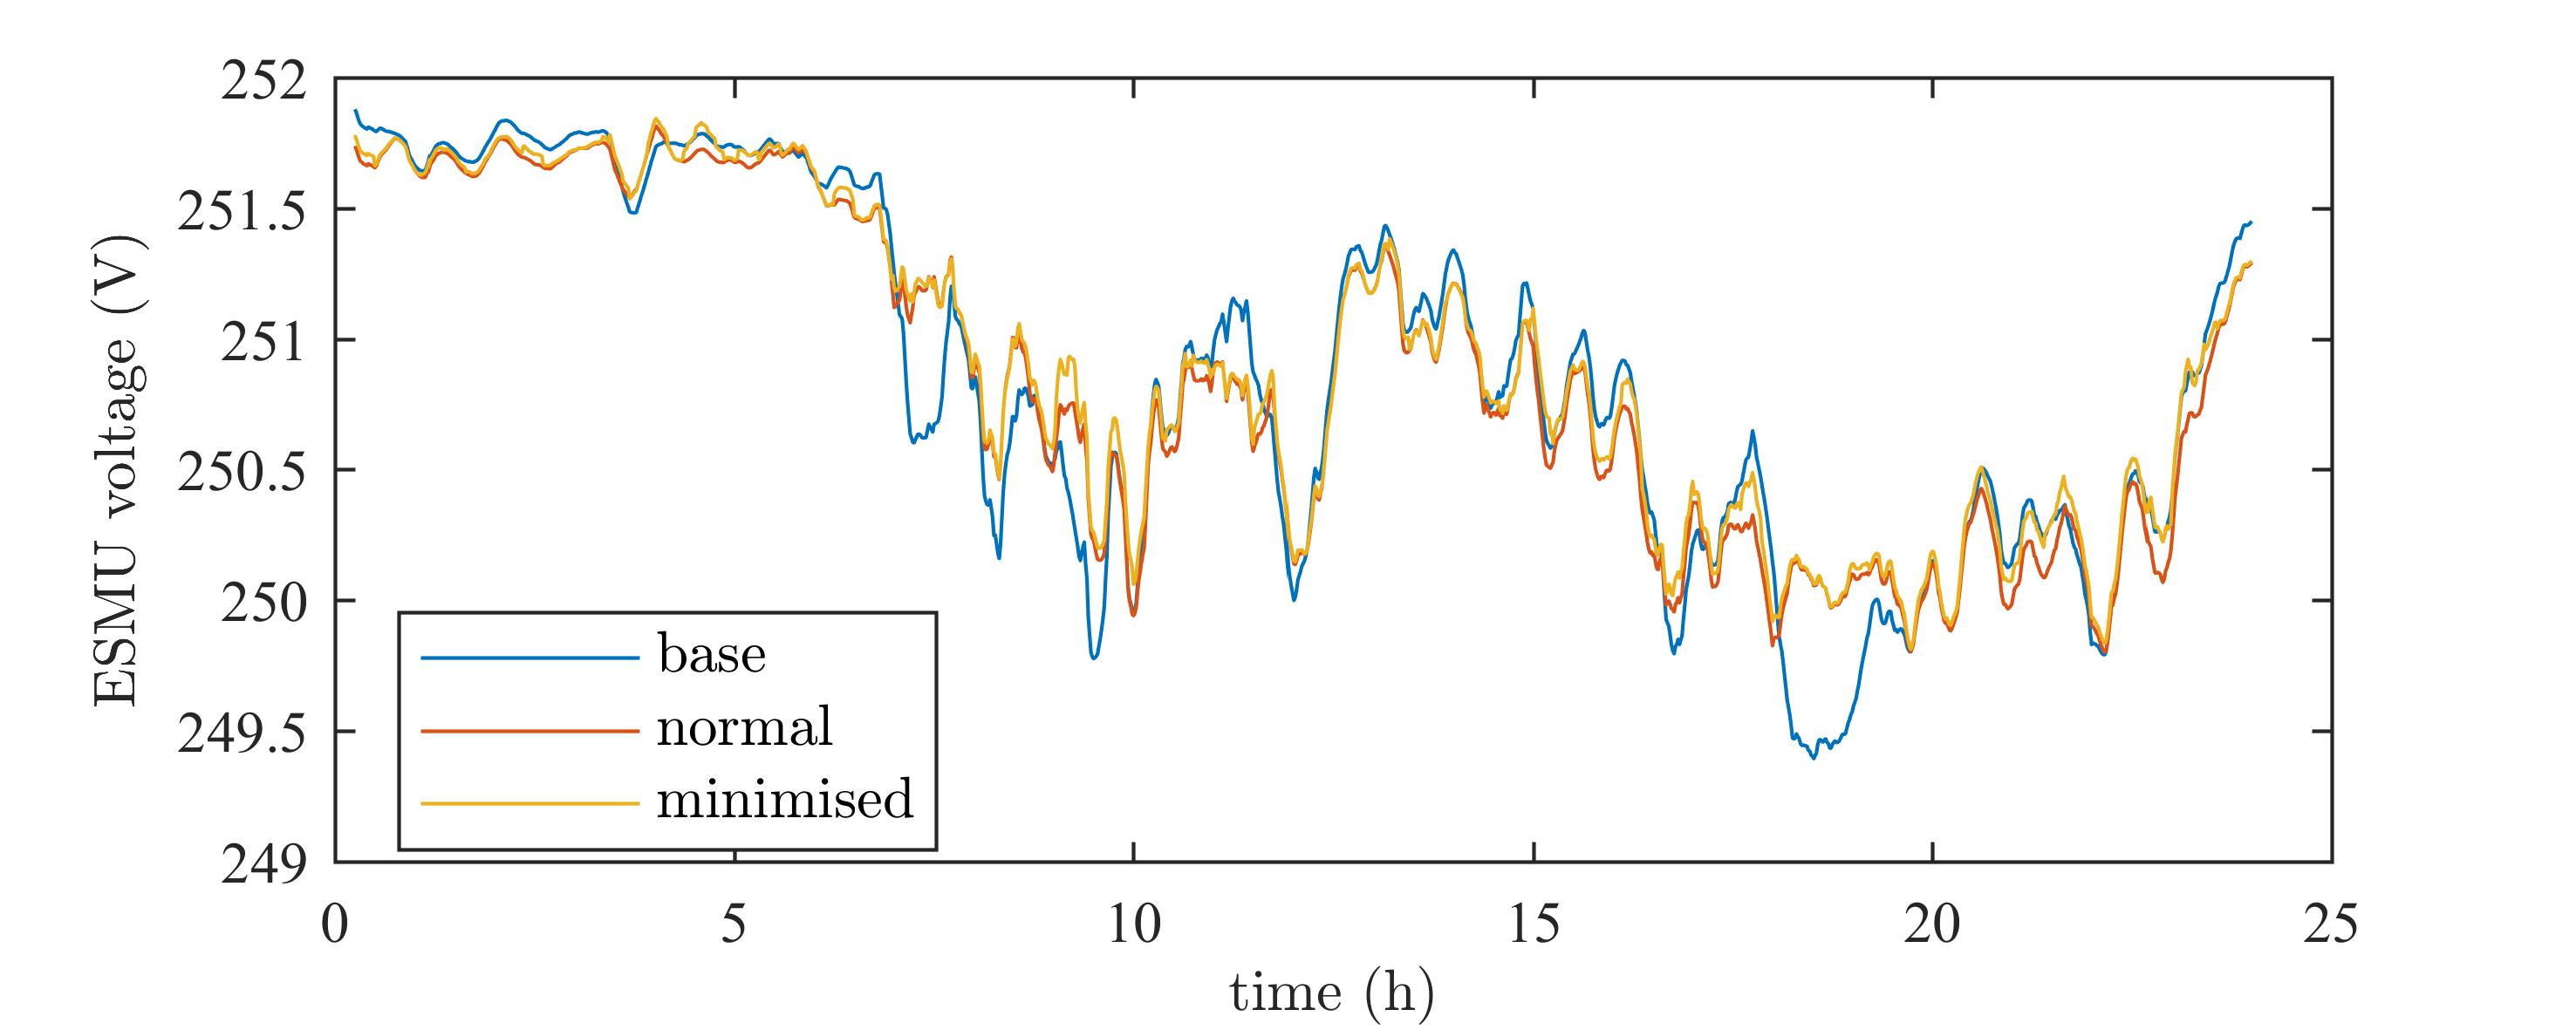
\includegraphics{_chapter1/fig/results/ts-esmu-voltages_}%
		\label{ch1:subfig:ts-esmu-voltage}%
	}\\
%	\vspace{5mm}
	\subfloat[Cost associated with the minimisation of the ESMU's PCC voltage deviation]{%
		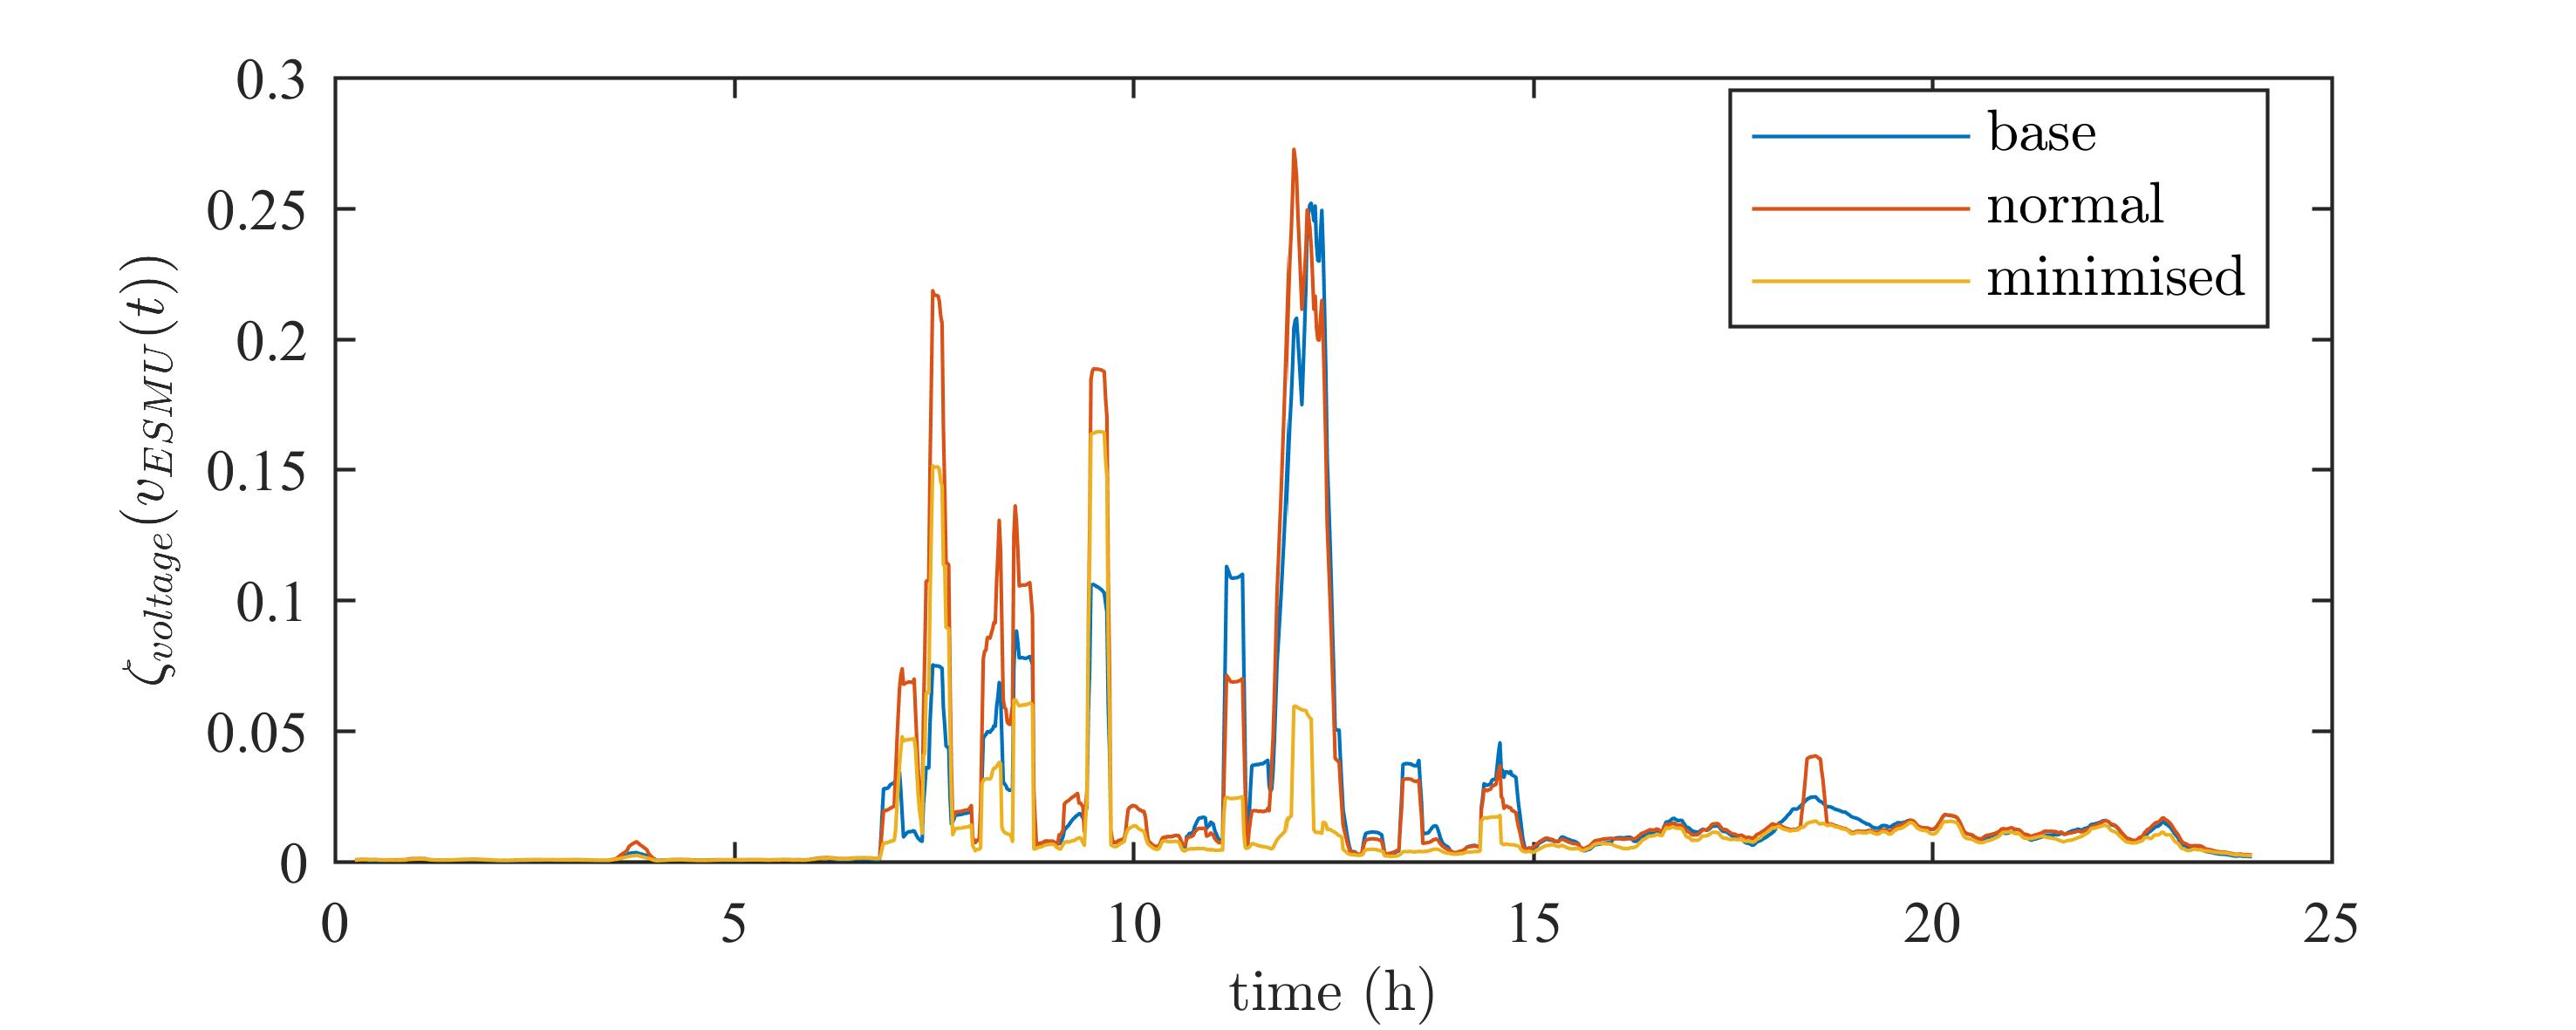
\includegraphics{_chapter1/fig/results/ts-esmu-voltages}%
		\label{ch1:subfig:ts-esmu-voltage-cost}%
	}
\caption{Voltage level modifications as noted at the ESMU's PCC by adjusting its schedule}
\label{ch1:fig:ts-esmu-voltages}
\end{figure}

In this figure the \textit{base} and \textit{normal} case's voltage profiles are plotted alongside the \textit{minimisation} case for which voltage deviation is minimised.
The plot shows that during the night's light load (i.e. from 0:00 to 6:00) ESMU was able to boost its voltage towards the nominal feeder voltage.
This is also the case during the lighter load in the afternoon (i.e. between 12:00-14:00).
But during the rest of the day when network load increases, the ESMU is unable to reduce voltage deviation to match its PCC voltage with the network's nominal substation voltage.
The reason behind this behaviour is that the ESMU has allocated its resources to serve for the underlying half-hourly ESMU schedule.
Therefore the remaining resources that could provide voltage support during periods of low demand become limited during periods of high demand.
Combined with the fact that the LV distribution networks are more resistive than inductive (i.e. unlike HV transmission networks), adjustments using the ESMU's reactive powers to stabilise voltage levels has an even smaller impact.
Nonetheless, due to some continuous yet small availability of power resource ESMU is able to boost voltages to some extent at all times.
In Figure~\ref{ch1:subfig:ts-esmu-voltage-cost} this can be seen since the associated cost has always been reduced in comparison to the \textit{base} and \textit{normal} cases.

The ability to support voltage levels at the ESMU's PCC is interesting, yet supporting voltage levels at all buses throughout the network is more relevant since some of these buses are linked to customers for which it is essential to maintain a constant voltage level.
Therefore, the following results assess both the highest and lowest voltage level that is recorded throughout the network.

\begin{figure}\centering
	\subfloat[Highest and lowest voltage levels that were recorded throughout the network when minimising the worst voltage deviation \hl{(nominal substation voltage is 252V)}]{%
		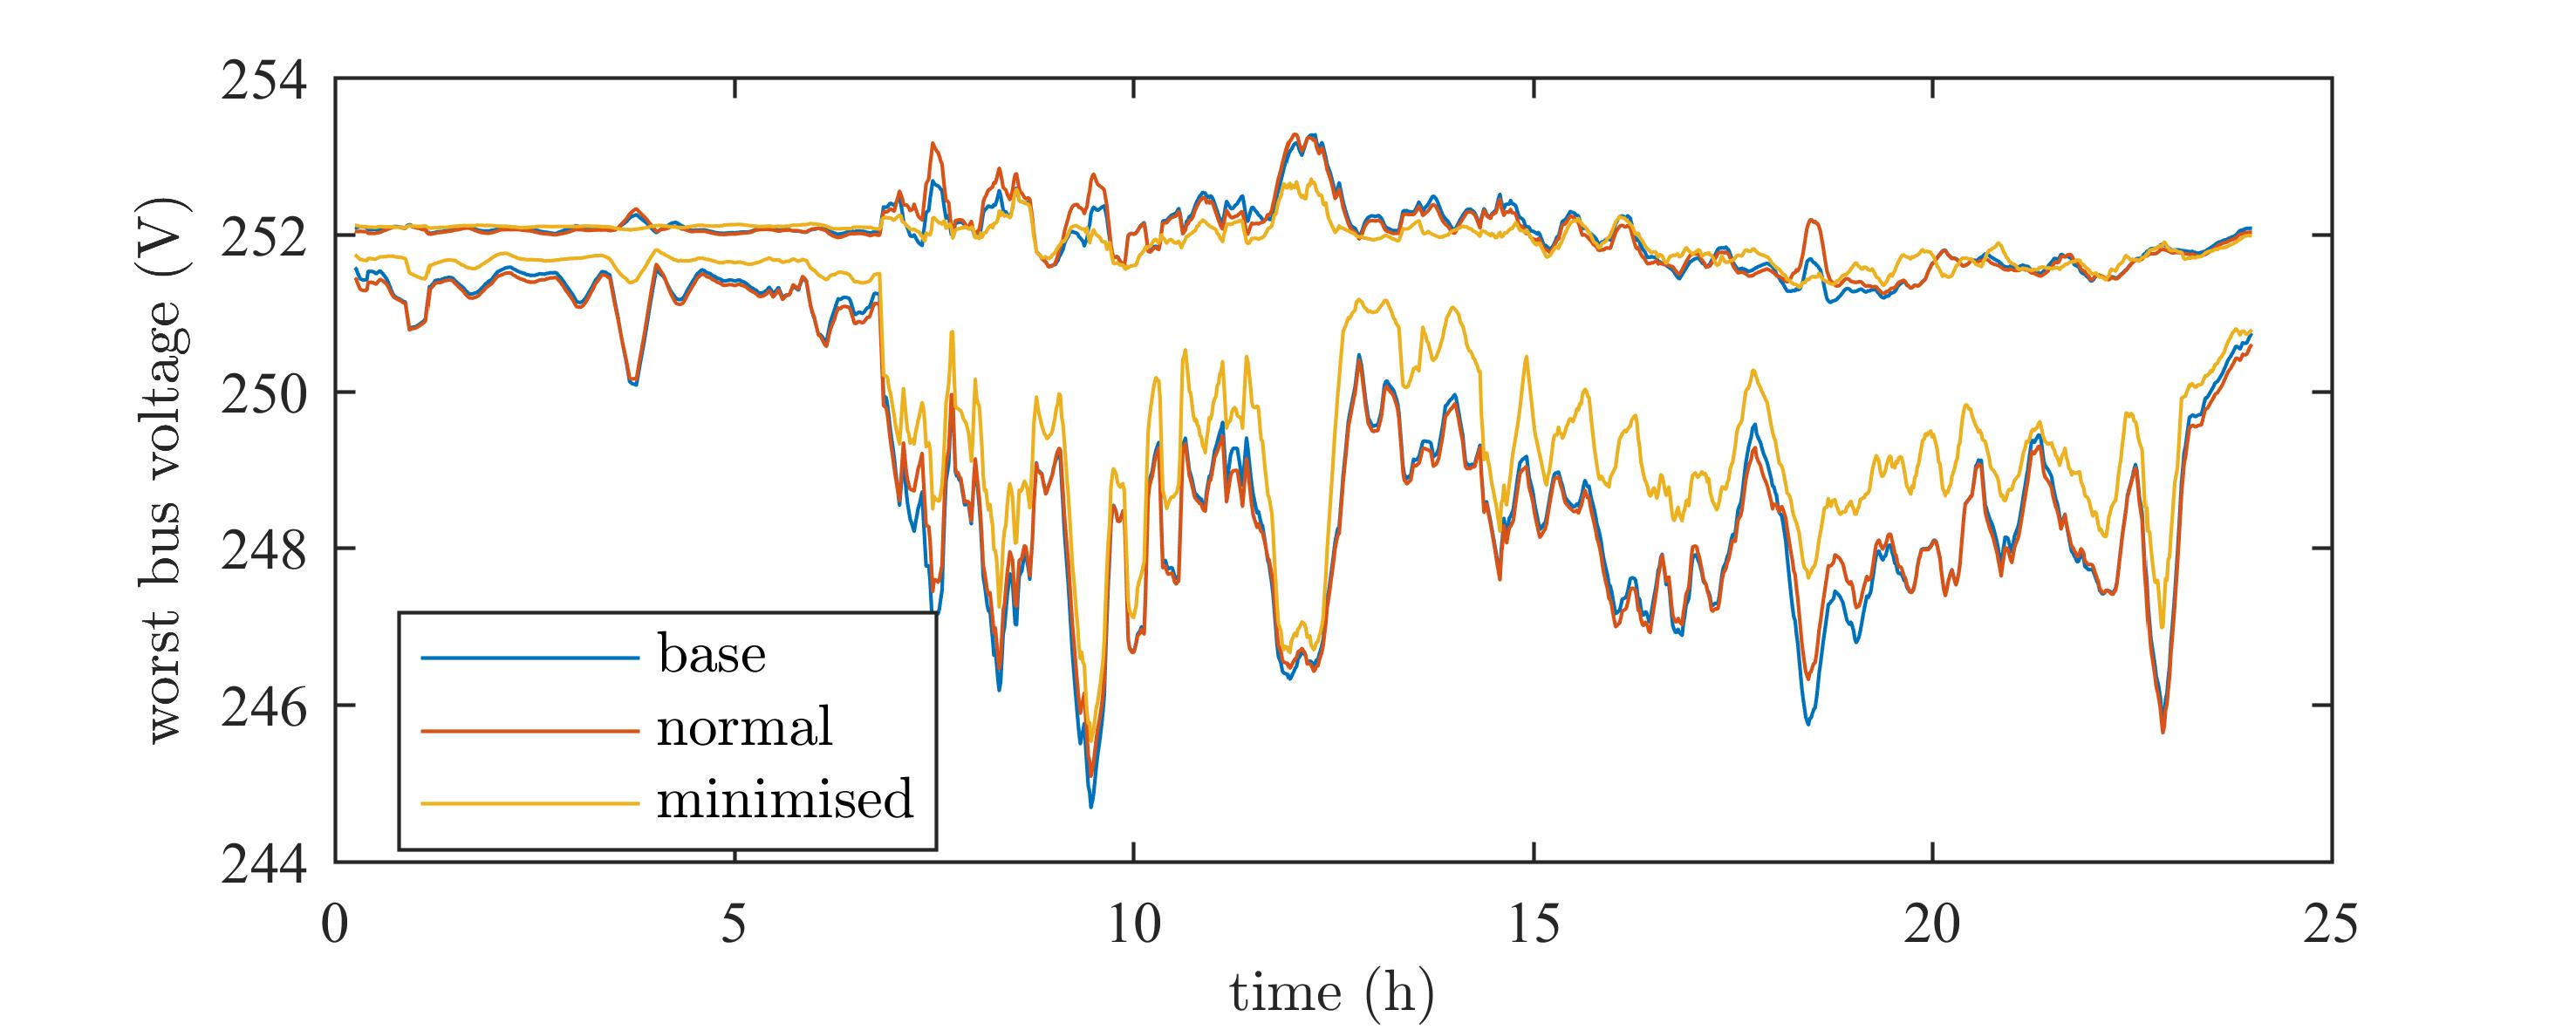
\includegraphics{_chapter1/fig/results/ts-all-voltages_}%
		\label{ch1:subfig:ts-all-voltages}%
	}\\
%	\vspace{5mm}
	\subfloat[Cost associated with the worst voltage deviation throughout the entire network]{%
		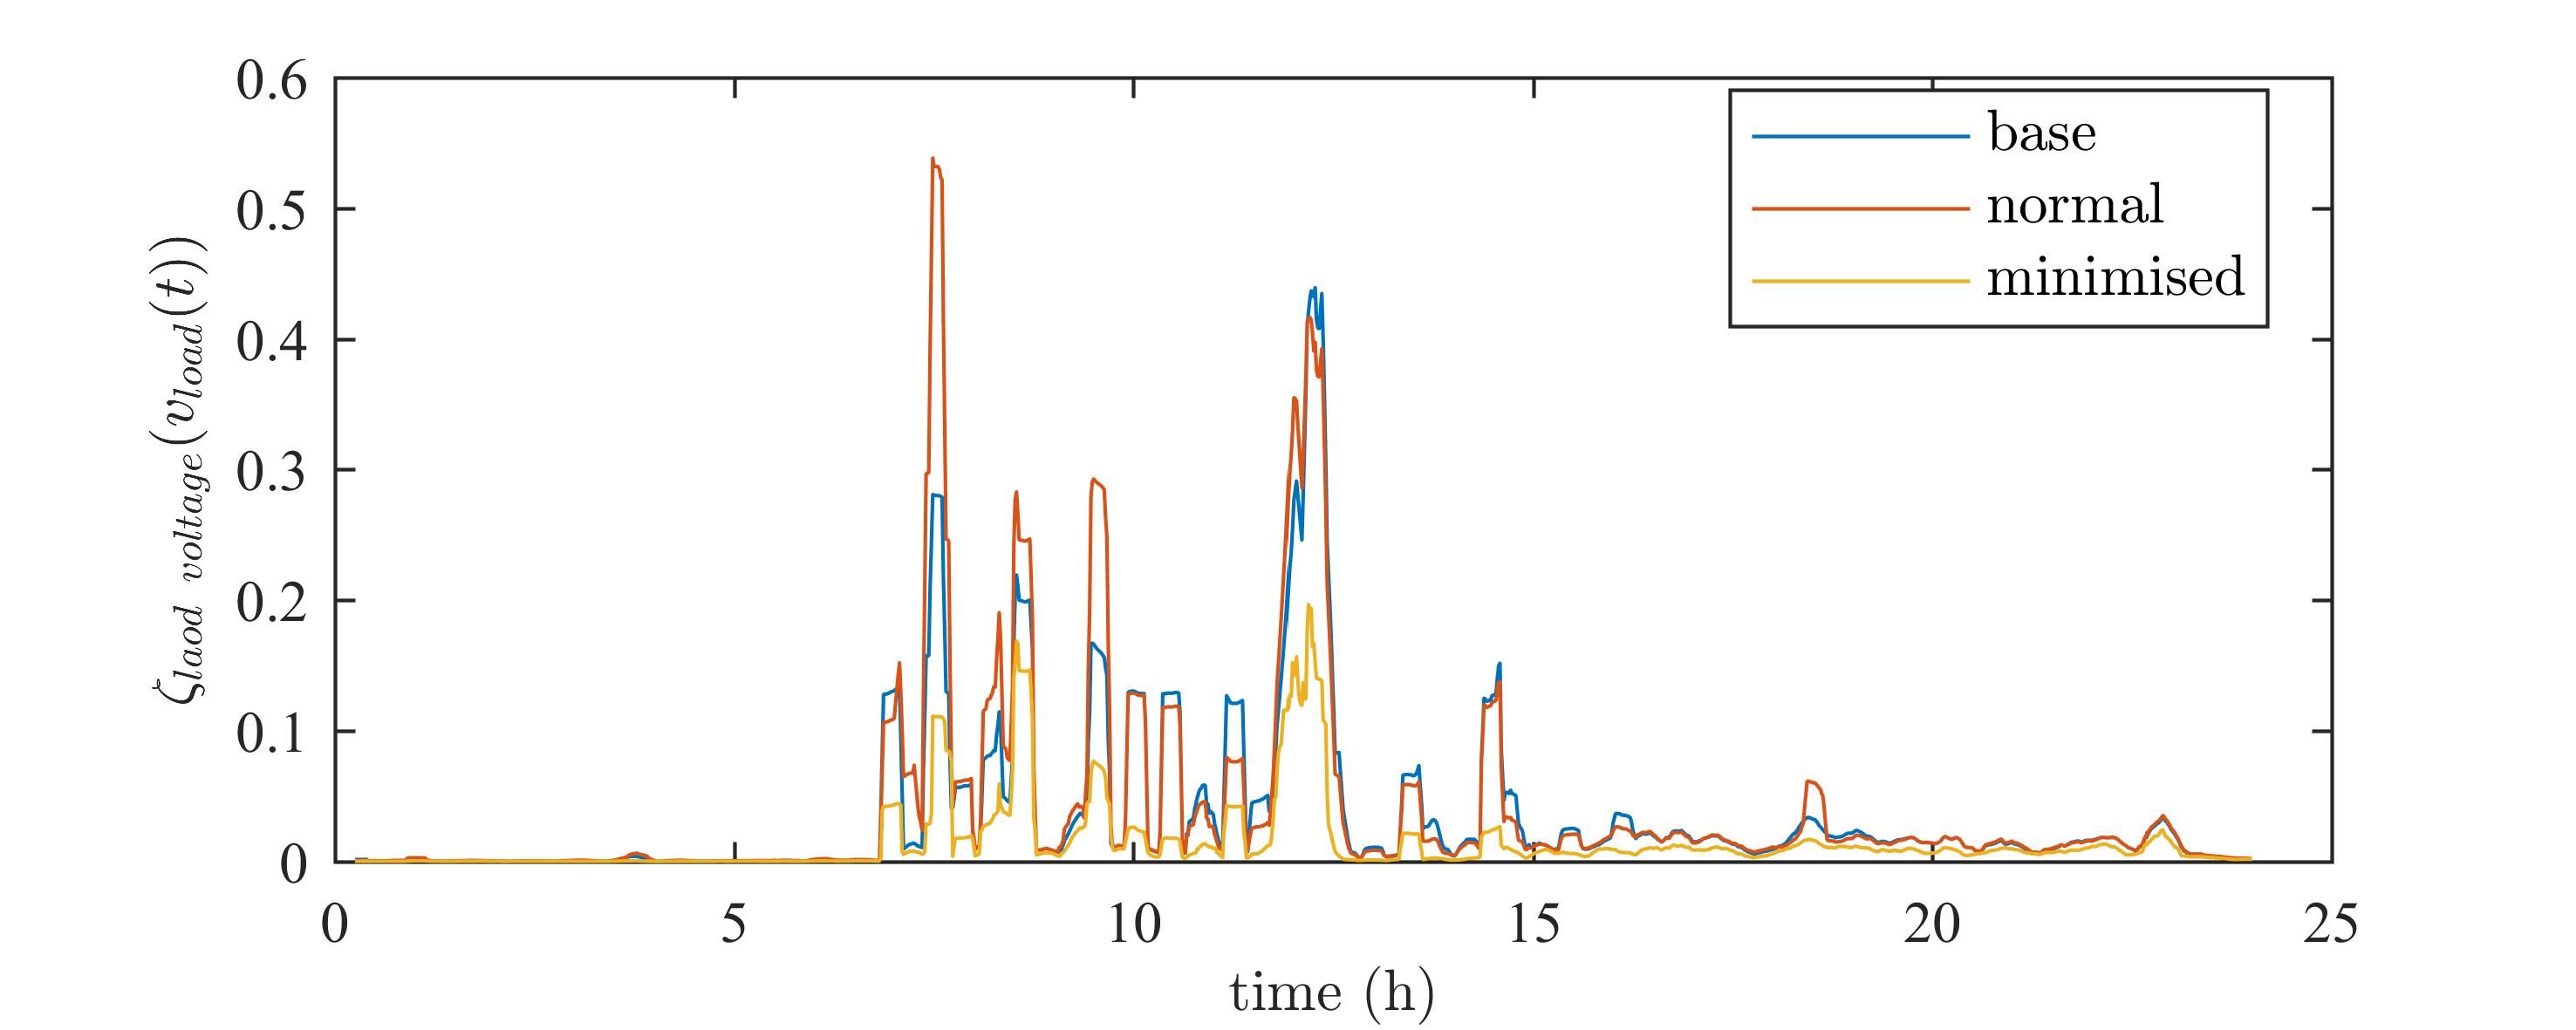
\includegraphics{_chapter1/fig/results/ts-all-voltages}%
		\label{ch1:subfig:ts-all-voltages-cost}%
	}
\caption{Voltage level improvements at all buses in the entire distribution network due to the ESMU schedule adjustment.}
\label{ch1:fig:ts-all-voltages}
\end{figure}

In Figure~\ref{ch1:subfig:ts-all-voltages}, despite no voltage violations taking place due to the already boosted substation voltage, the ESMU's positive impact can be observed.
Here the difference between highest and lowest bus voltage of the network is indicated by two lines of the same color. It is this difference that is noticeably reduced and their average voltage is brought closer to a nominal voltage level.
The ESMU's function to support the network in providing more stable voltage levels at customer endpoints is therefore met.
This fact is also supported by the associated cost plot in Figure~\ref{ch1:subfig:ts-all-voltages-cost} where a reduction in cost can be observed throughout the entire simulated day.

\begin{figure}\centering
	\subfloat[Network's highest and lowest phase power demand when phase unbalance was minimised]{%
		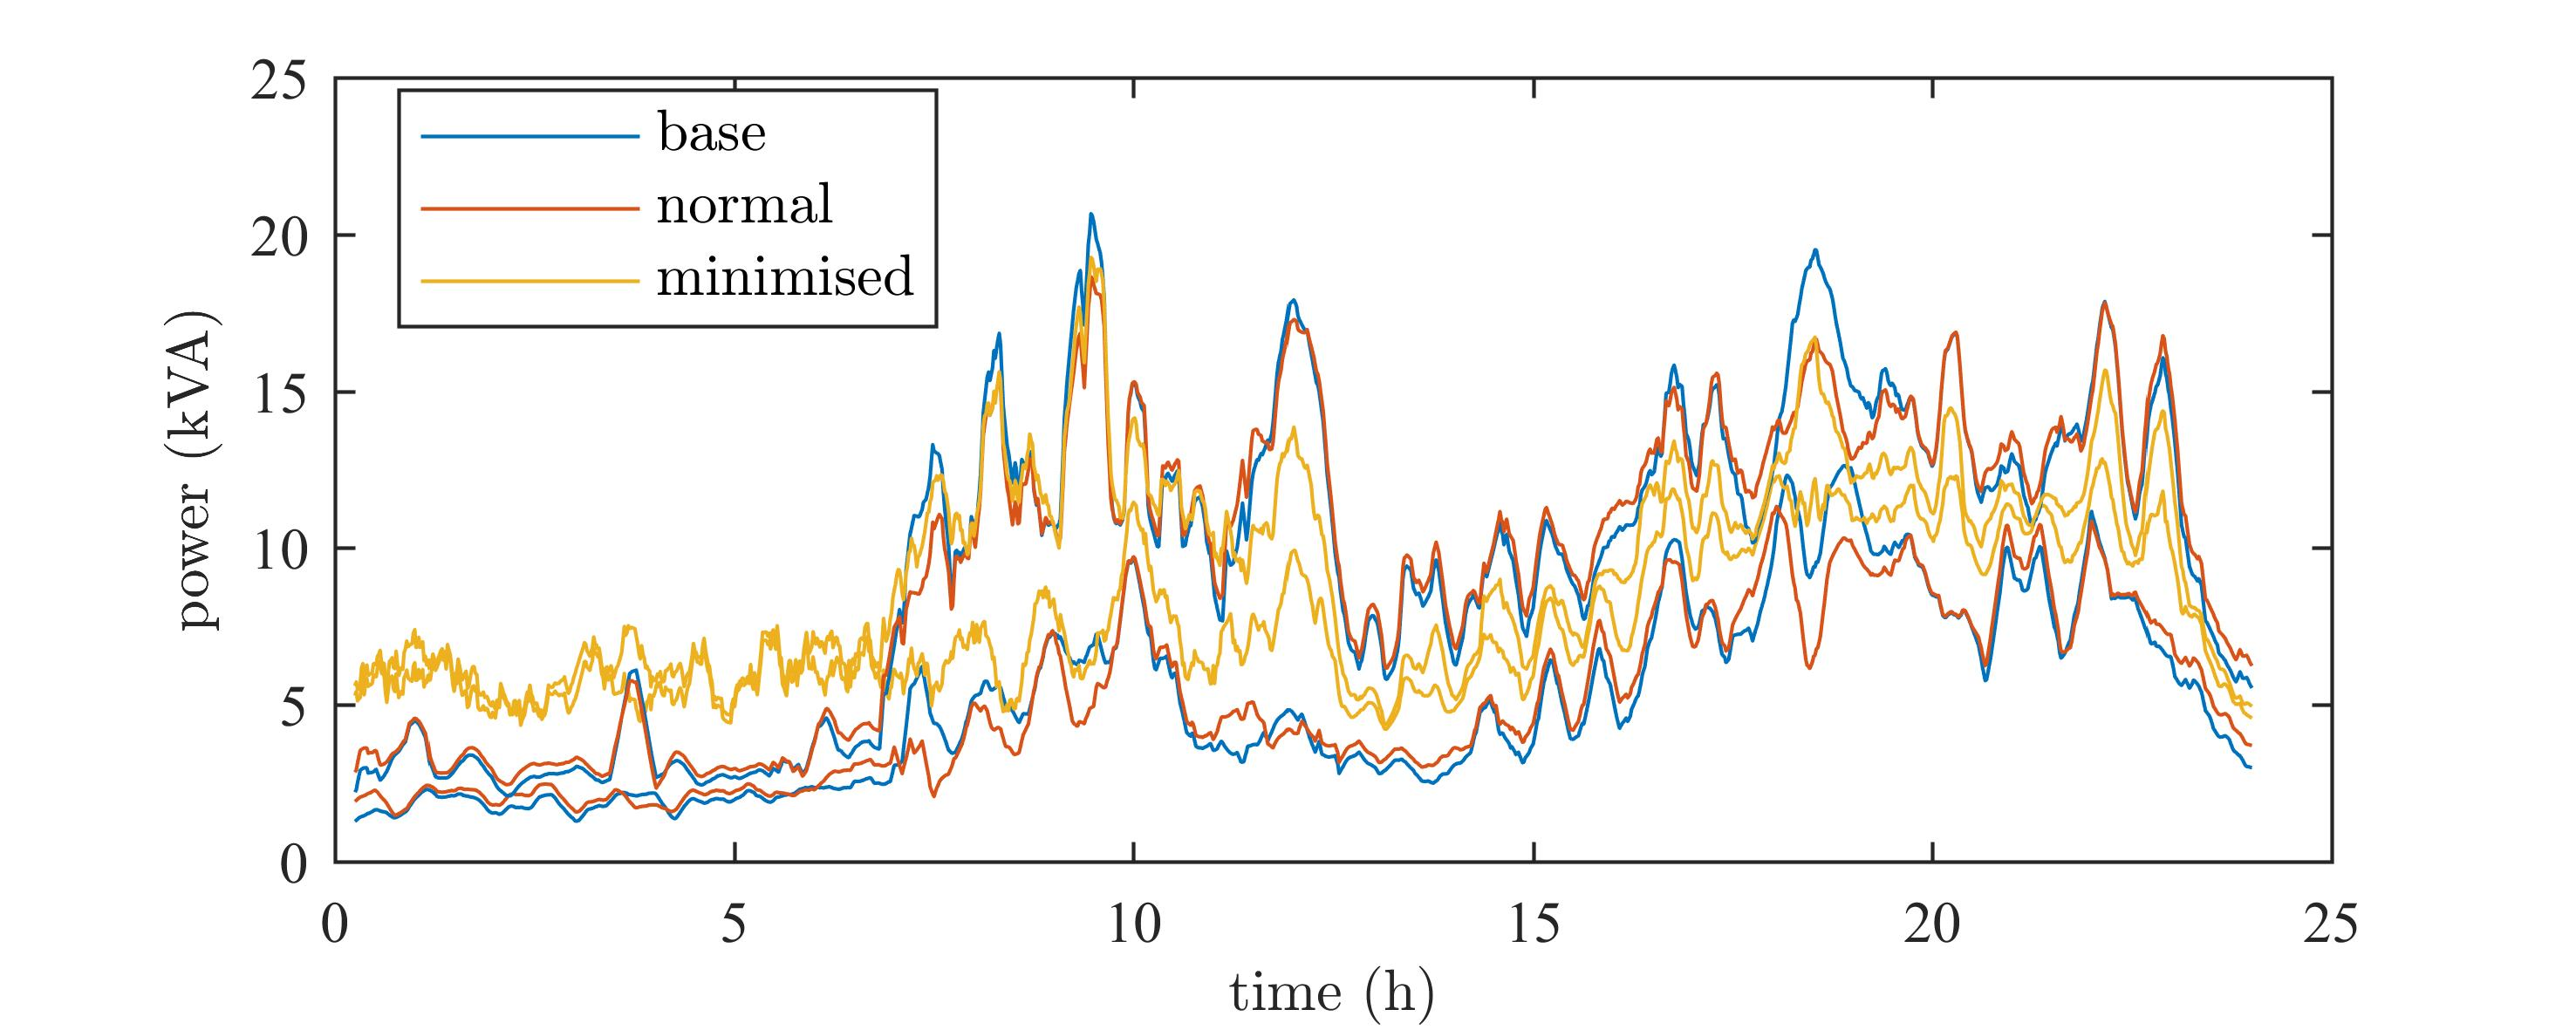
\includegraphics{_chapter1/fig/results/ts-phase-unbalance_}%
		\label{ch1:subfig:ts-phase-unbalance}%
	}\\
%	\vspace{5mm}
	\subfloat[Cost associated with the network's phase unbalance]{%
		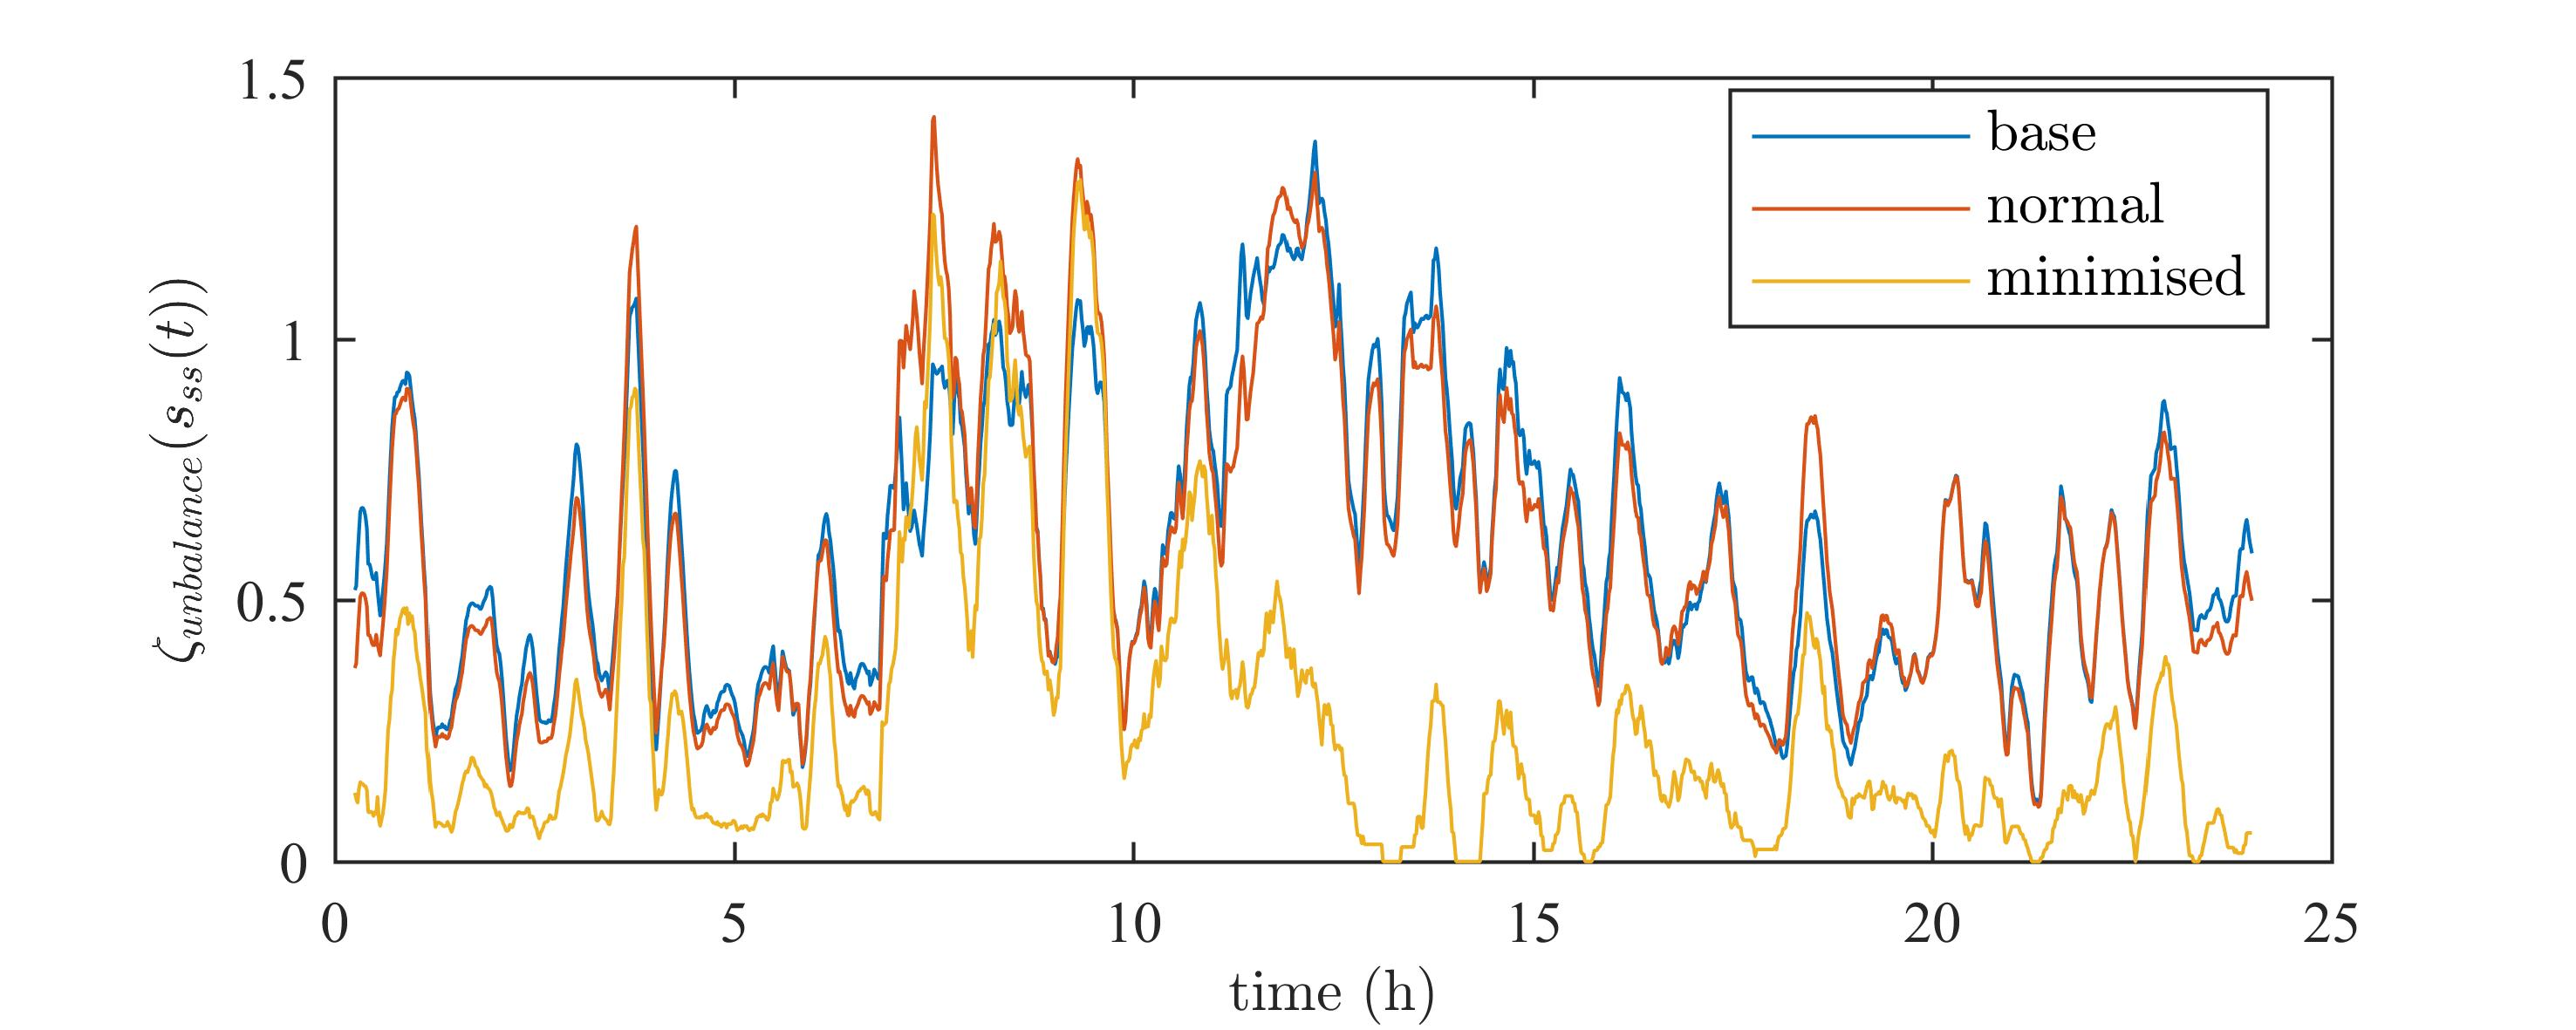
\includegraphics{_chapter1/fig/results/ts-phase-unbalance}%
		\label{ch1:subfig:ts-phase-unbalance-cost}%
	}
\caption{Reduction of the network's phase unbalance due to the adjustment of the ESMU schedule.}
\label{ch1:fig:ts-phase-unbalance}
\end{figure}

Beside providing stable voltage levels, power quality should also be upheld to assure that distribution networks operate as efficient as possible.
The first power related parameter that indicates network efficiency is phase unbalance.
In Figure~\ref{ch1:subfig:ts-phase-unbalance} the power value of the highest and lowest loaded corresponding phases is plotted over time.
At all times the sub-half-hourly adjustments of the ESMU's schedule did reduce the underlying phase imbalance.
This was achieved by redistributing power from the most loaded phase to the least loaded phases; hence utilising the unused capacity of the lighter loaded phases.
As expected, the associated cost has been noticeably lowered in comparison to the \textit{base} and \textit{normal} cases.
It should however be noted that phase balancing during the morning hours is predominantly achieved by using reactive power injection and absorption.
This can be seen by the similar yet increased phase loadings between 0:00 and 7:00.
Therefore the tradeoff between adding additional strain onto the network versus balancing phases has to be taken into account.
One such strain that is being put onto the network is increased neutral power flow due to phasor misalignment.

\begin{figure}\centering
	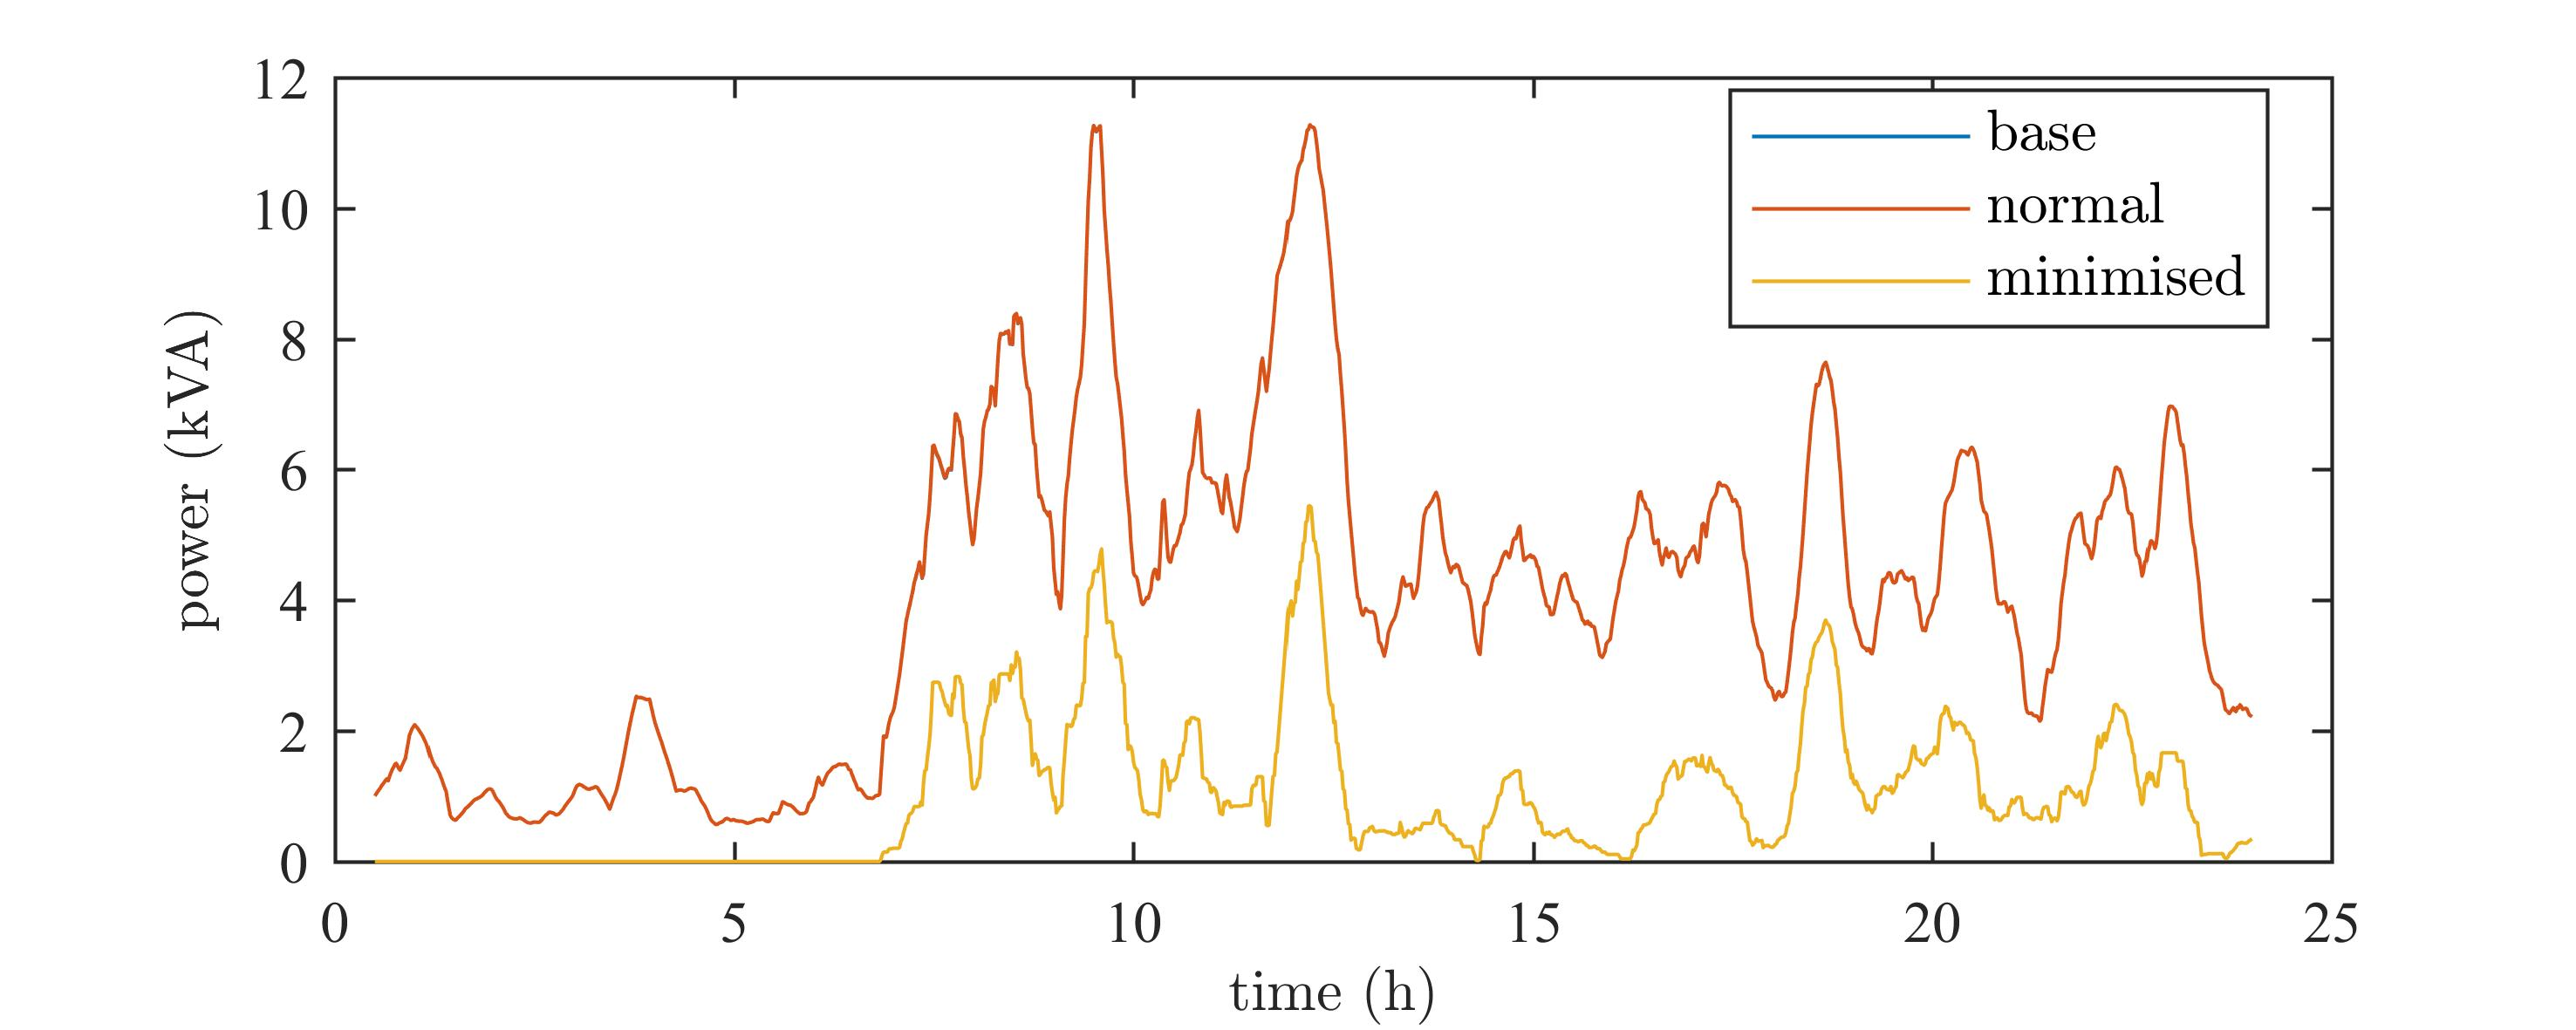
\includegraphics[width=\textwidth]{_chapter1/fig/ts-neutral-power-2}
\caption{Neutral power reduction due to the ESMU schedule adjustments}
\label{ch1:fig:ts-neutral-power}
\end{figure}

For the results that are plotted in Figure~\ref{ch1:fig:ts-neutral-power}, neutral power flow is minimised through the adjustment of ESMU powers.
It can be seen that for the \textit{normal} case neutral power is not affected at all.
Reason for this result is the choice of evenly assigning the scheduled ESMU power to all three phases.
Therefore neither phase unbalance nor loading of the neutral conductor is being taken into account.
For the \textit{minimisation} case however, loading of the neutral conductor is successfully reduced in comparison to both the \textit{normal} and \textit{base} case.

\begin{figure}\centering
	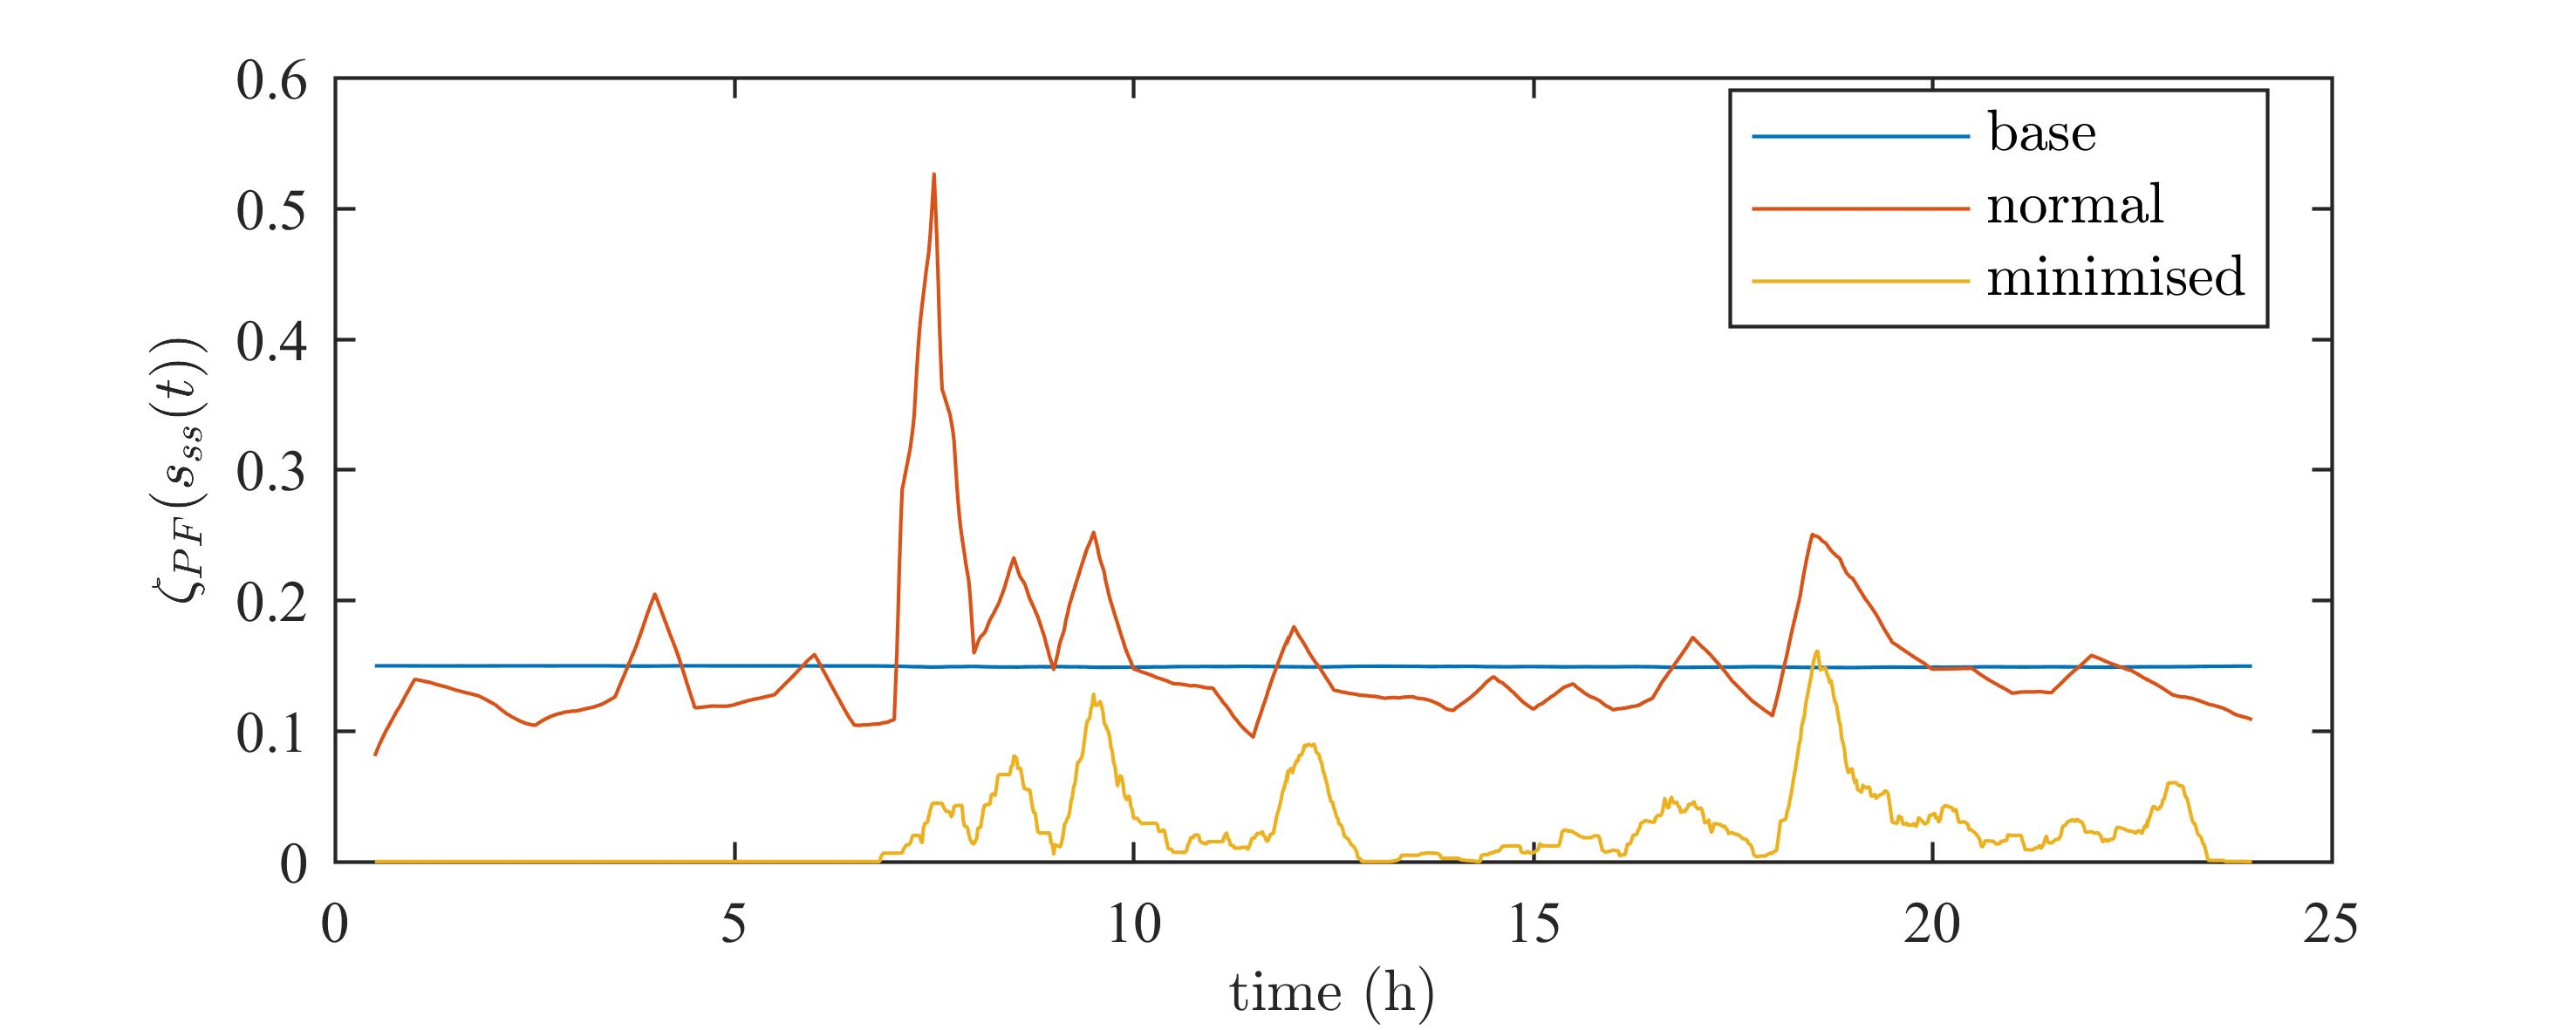
\includegraphics[width=\textwidth]{_chapter1/fig/ts-power-factor}
\caption{Power factor cost improvements due to the adjustment of the ESMU schedule}
\label{ch1:fig:ts-power-factor}
\end{figure}

Unlike neutral phase unbalance and neutral loading, power factor on the other hand is impacted just by introducing the half-hourly ESMU schedule as shown in Figure~\ref{ch1:fig:ts-power-factor}.
Whilst the choice of a static power factor for all loads in the \textit{base} case resulted in a constant power throughout the day, half-hourly ESMU intervention in the \textit{normal} case results in a noticeable power factor variation.
This variation is however successfully reduced throughout the entire day for the \textit{minimisation} case in comparison to the \textit{normal} case.

\begin{figure}\centering
	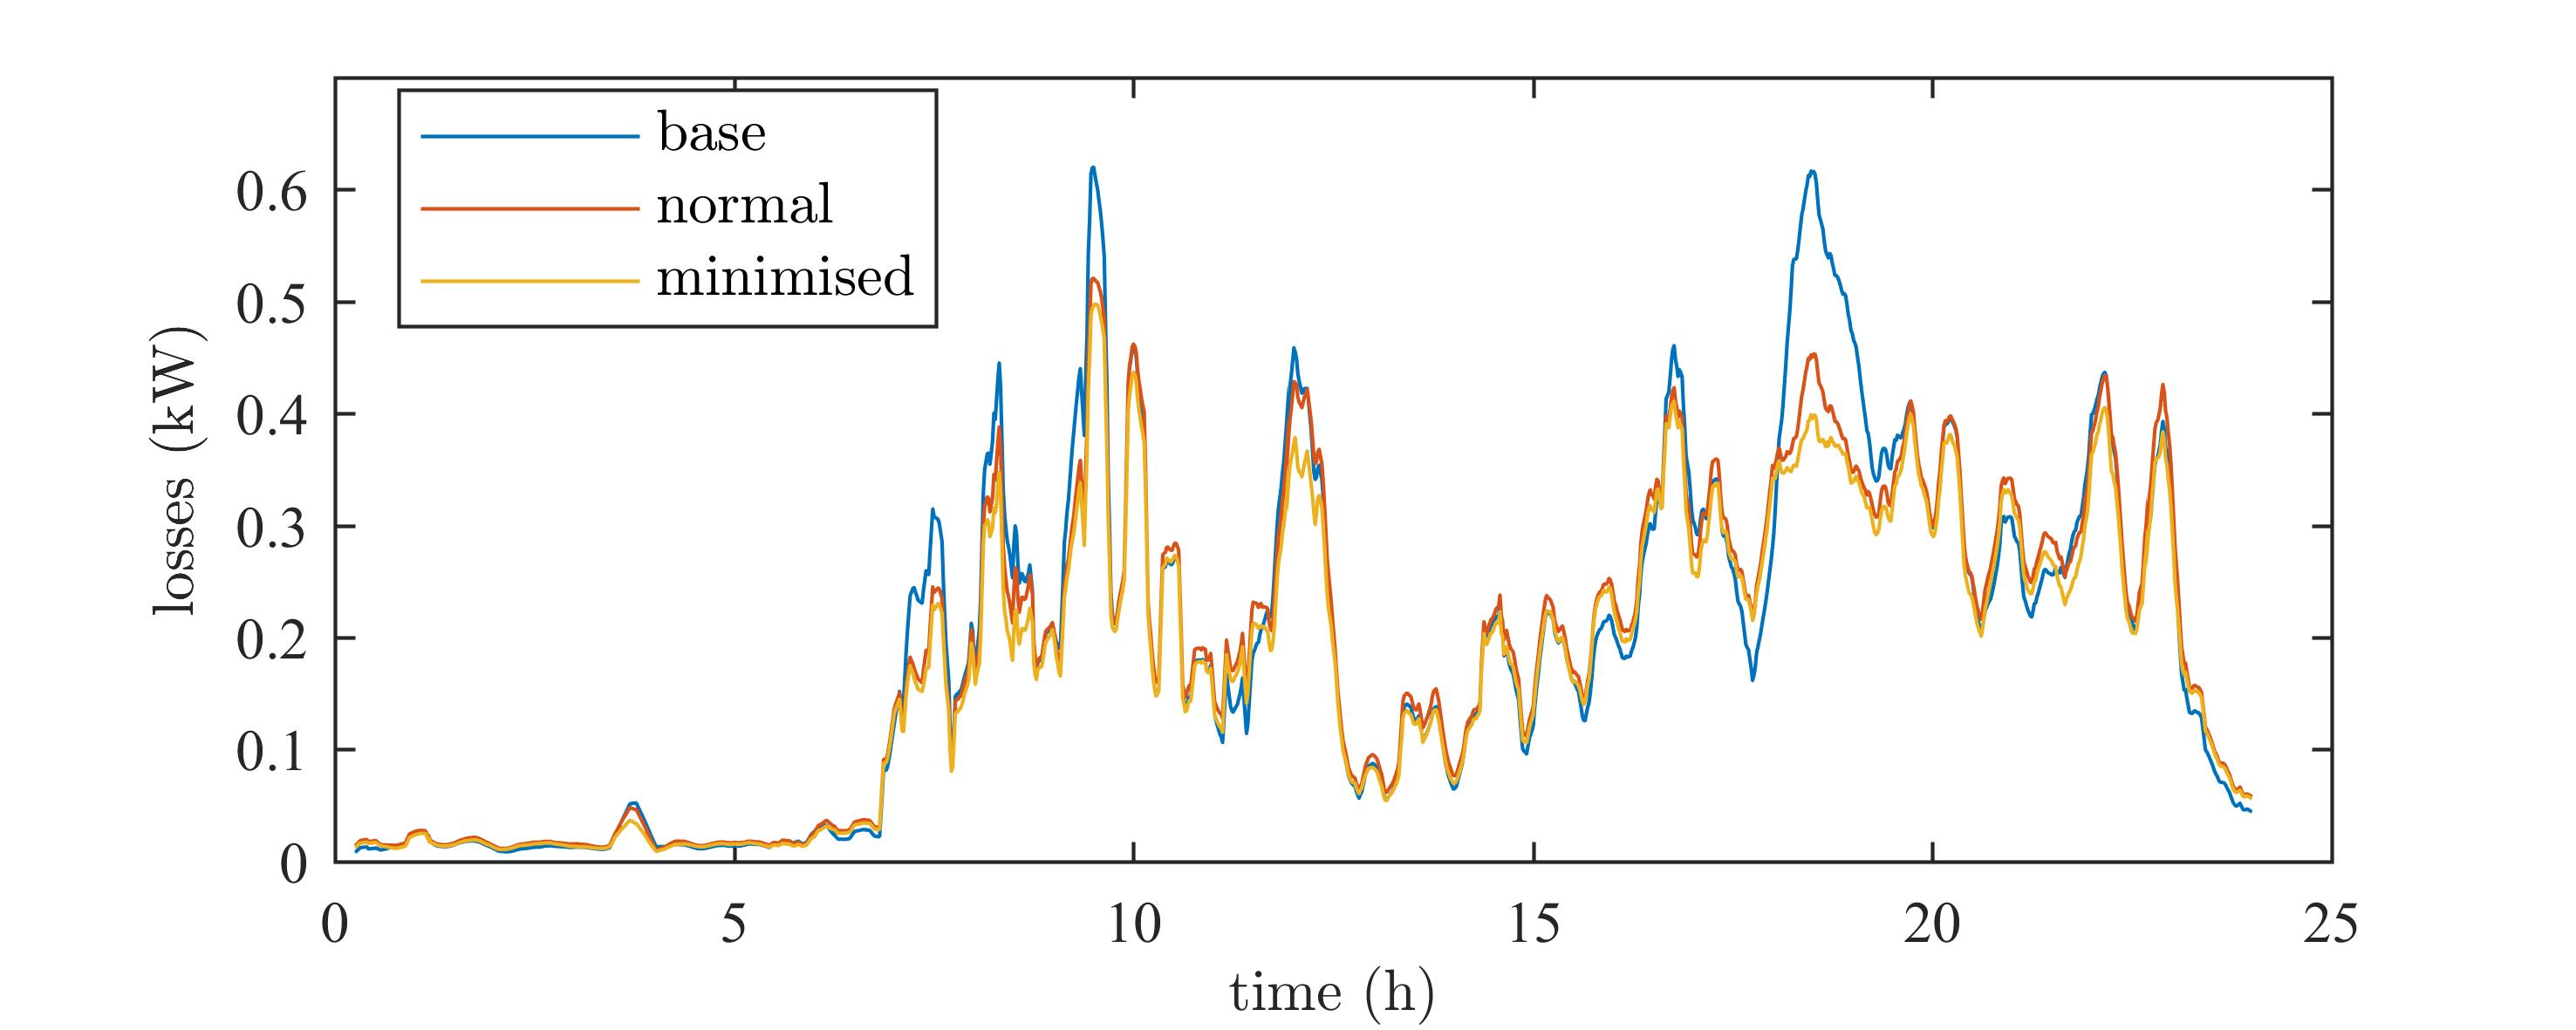
\includegraphics{_chapter1/fig/results/ts-losses_}
\caption{Instantaneous losses of the distribution network when adjusting the ESMU schedule in order to reduce the former \hl{(energy lost: 4.55kWh for base; 4.47kWh for normal; 4.19kWh for minimised)}.}
\label{ch1:fig:ts-losses}
\end{figure}

The final parameter that indicates system efficiency are the distribution losses.
Figure~\ref{ch1:fig:ts-losses} shows the reduction in distribution losses that were achieved when adjusting the ESMU powers accordingly.
In fact, when compared to the \textit{base} case, the \textit{normal} case lead to a daily energy saving of 0.07kWh.
The \textit{minimised} case however reduced daily losses by 0.36kWh.
This equates to more than five times the energy saving that can be achieved simply by adjusting the ESMU's power injection and absorption behaviour.
Although this amount of energy seems negligibly small these saving can amount to a noticeable level of savings on a national scale which can potentially benefit the entire power network.
Nonetheless, measuring losses is difficult and costly which is why attempting to do so will likely outweigh the benefits that are shown above.

Instead, a better way of relieving stress from the power network is to minimise its assets utilisation by mitigating demand spikes that were taken into account in Equation~\ref{ch1:equ:scheduling-cost}.
However, since the ESMU was constraint to not deviate from its underlying half-hourly schedule only phase related demand differences can be addressed and the impact of correcting those phase differences is barely noticeable.
This limitation can be seen in Figure~\ref{ch1:fig:ts-all-line-utilisation}.

\begin{figure}\centering
	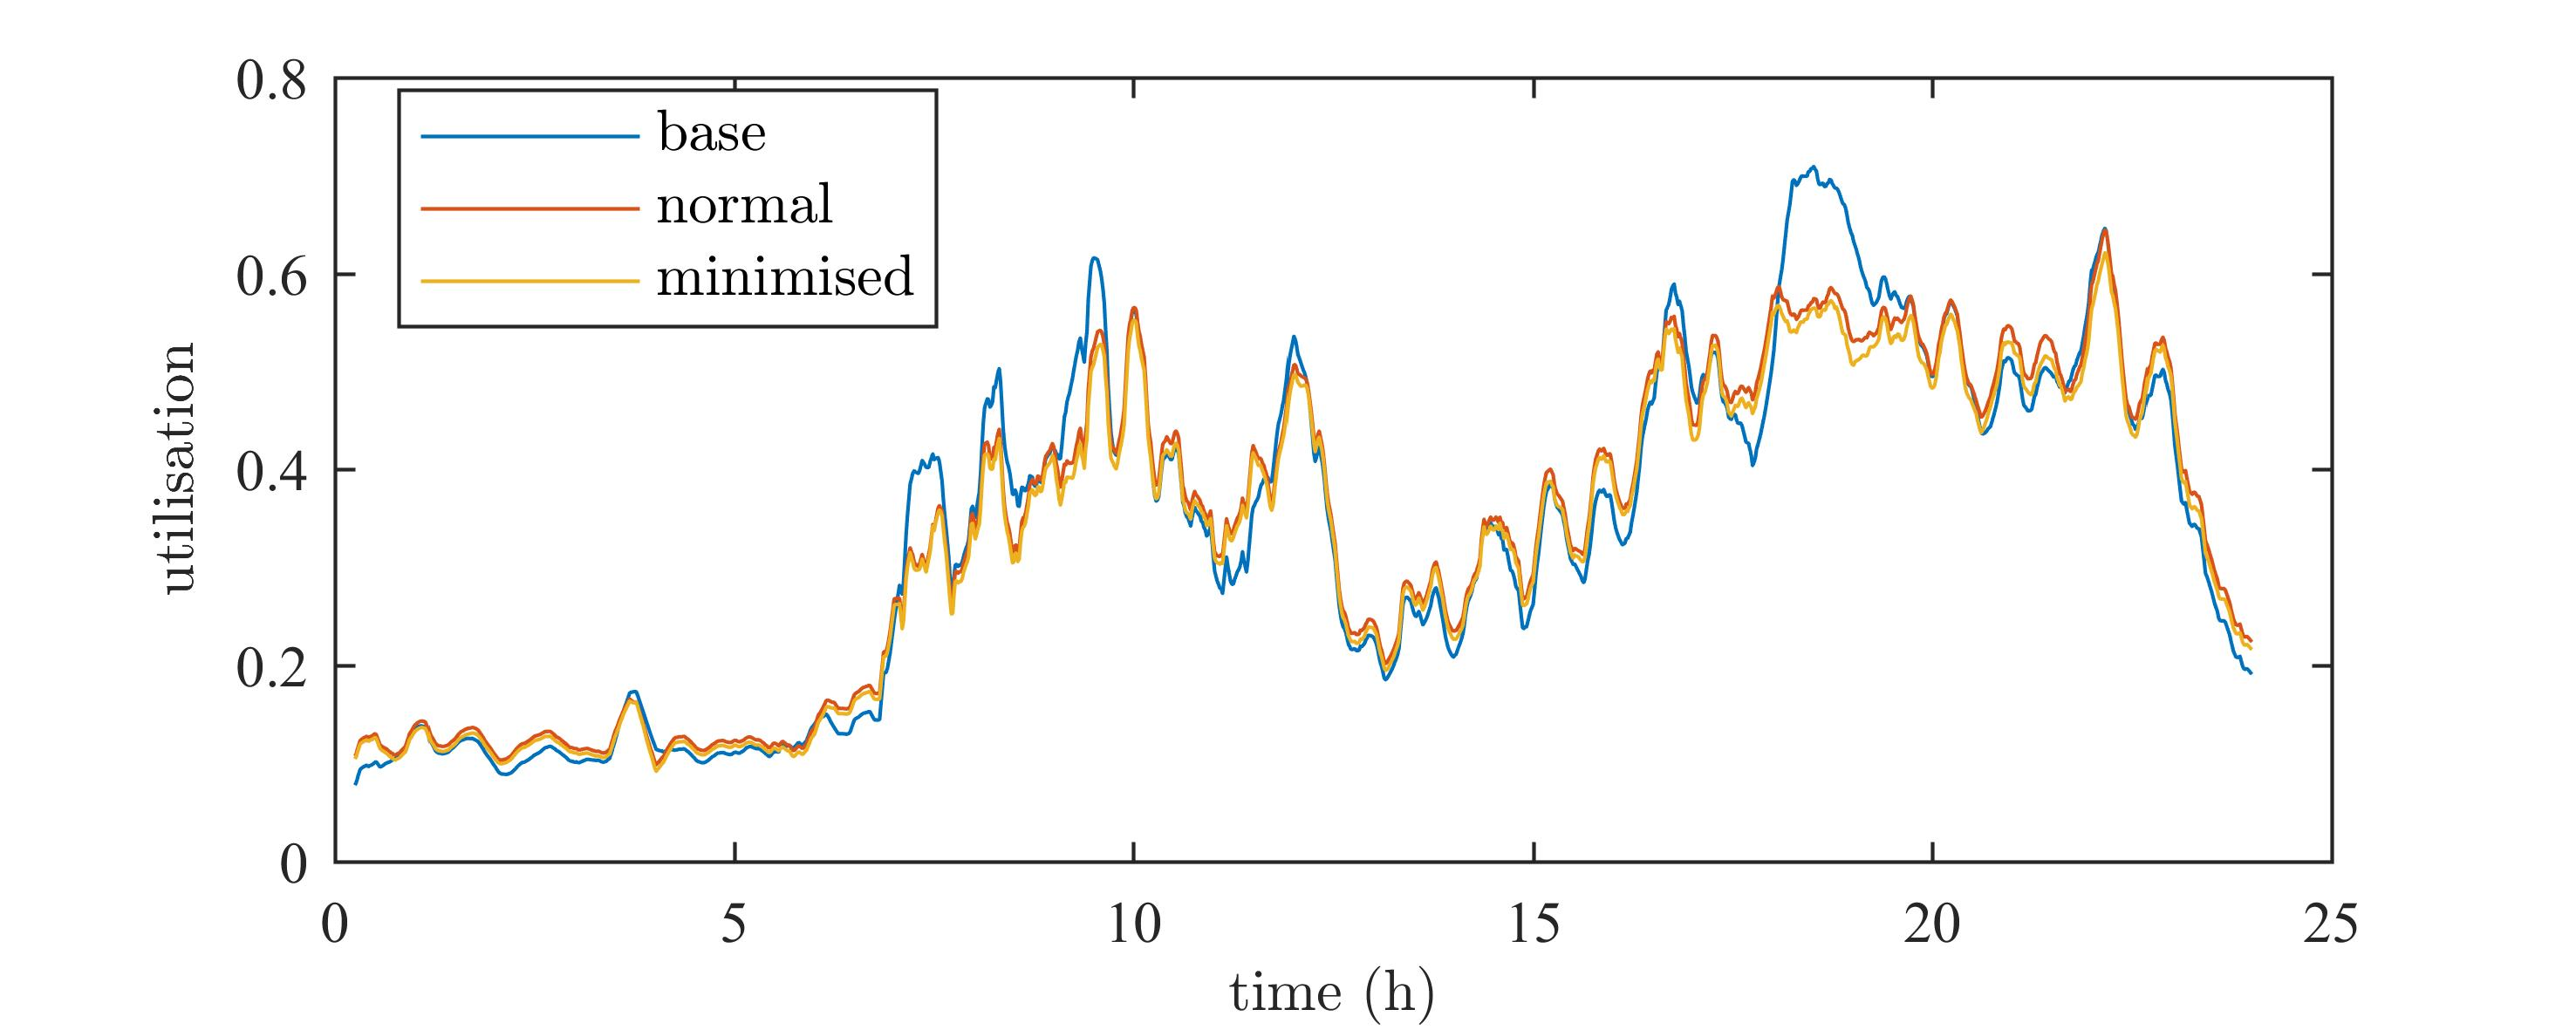
\includegraphics{_chapter1/fig/results/ts-all-line-utilisation_}
\caption{Improvement of the worst line utilisation across the entire network when adjusting the ESMU schedule correspondingly.}
\label{ch1:fig:ts-all-line-utilisation}
\end{figure}

Whilst the \textit{normal} case noticeably lowered some of the daily demand, power spikes after for example 9pm were not addressed at all.
Even the \textit{minimisation} case could barely reduce those spikes due to the constraining half-hourly schedule.
Nonetheless, throughout the entire day ESMU was still able to reduce line utilisation at the substation level; despite those improvements being relatively small in comparison to the impact in the \textit{normal} case.

\subsection{Difference Analysis}
\label{ch1:subsec:difference-analysis}

In order to gage whether the sub-half-hourly ESMU power adjustment results in a statistical difference in network performance, a box-plot was generated to compare each \textit{minimisation} with the corresponding \textit{normal} case.
Hence, the underlying data for each box-plot represents the difference between the \textit{minimisation} case's costs and the \textit{normal} case's costs, i.e. when operating without adjusting ESMU powers.
Therefore any positive difference in cost indicates an improvement to the system's performance whilst a negative difference would imply a worsening.
All cases are compared and plotted in Figure~\ref{ch1:fig:boxplot-overall-improvements}, and the complete set of box-plots (i.e. showing the ``cross-cost difference'') is included in Appendix~\ref{appx-a:ch1:additional-difference-analysis}.
On each of these box-plots, the central red mark indicates the median, and the bottom and top edges of the blue box indicate the 25$^\text{th}$ and 75$^\text{th}$ percentiles, respectively.
The whiskers extend to the most extreme data points not considered outliers, and the outliers are plotted individually using the red '$+$' symbol.
In Figure~\ref{ch1:fig:boxplot-overall-improvements} an individual axis, scaled at 10:1, is used for indicating the cost of neutral power to better visualise its distribution.

\begin{figure}\centering
	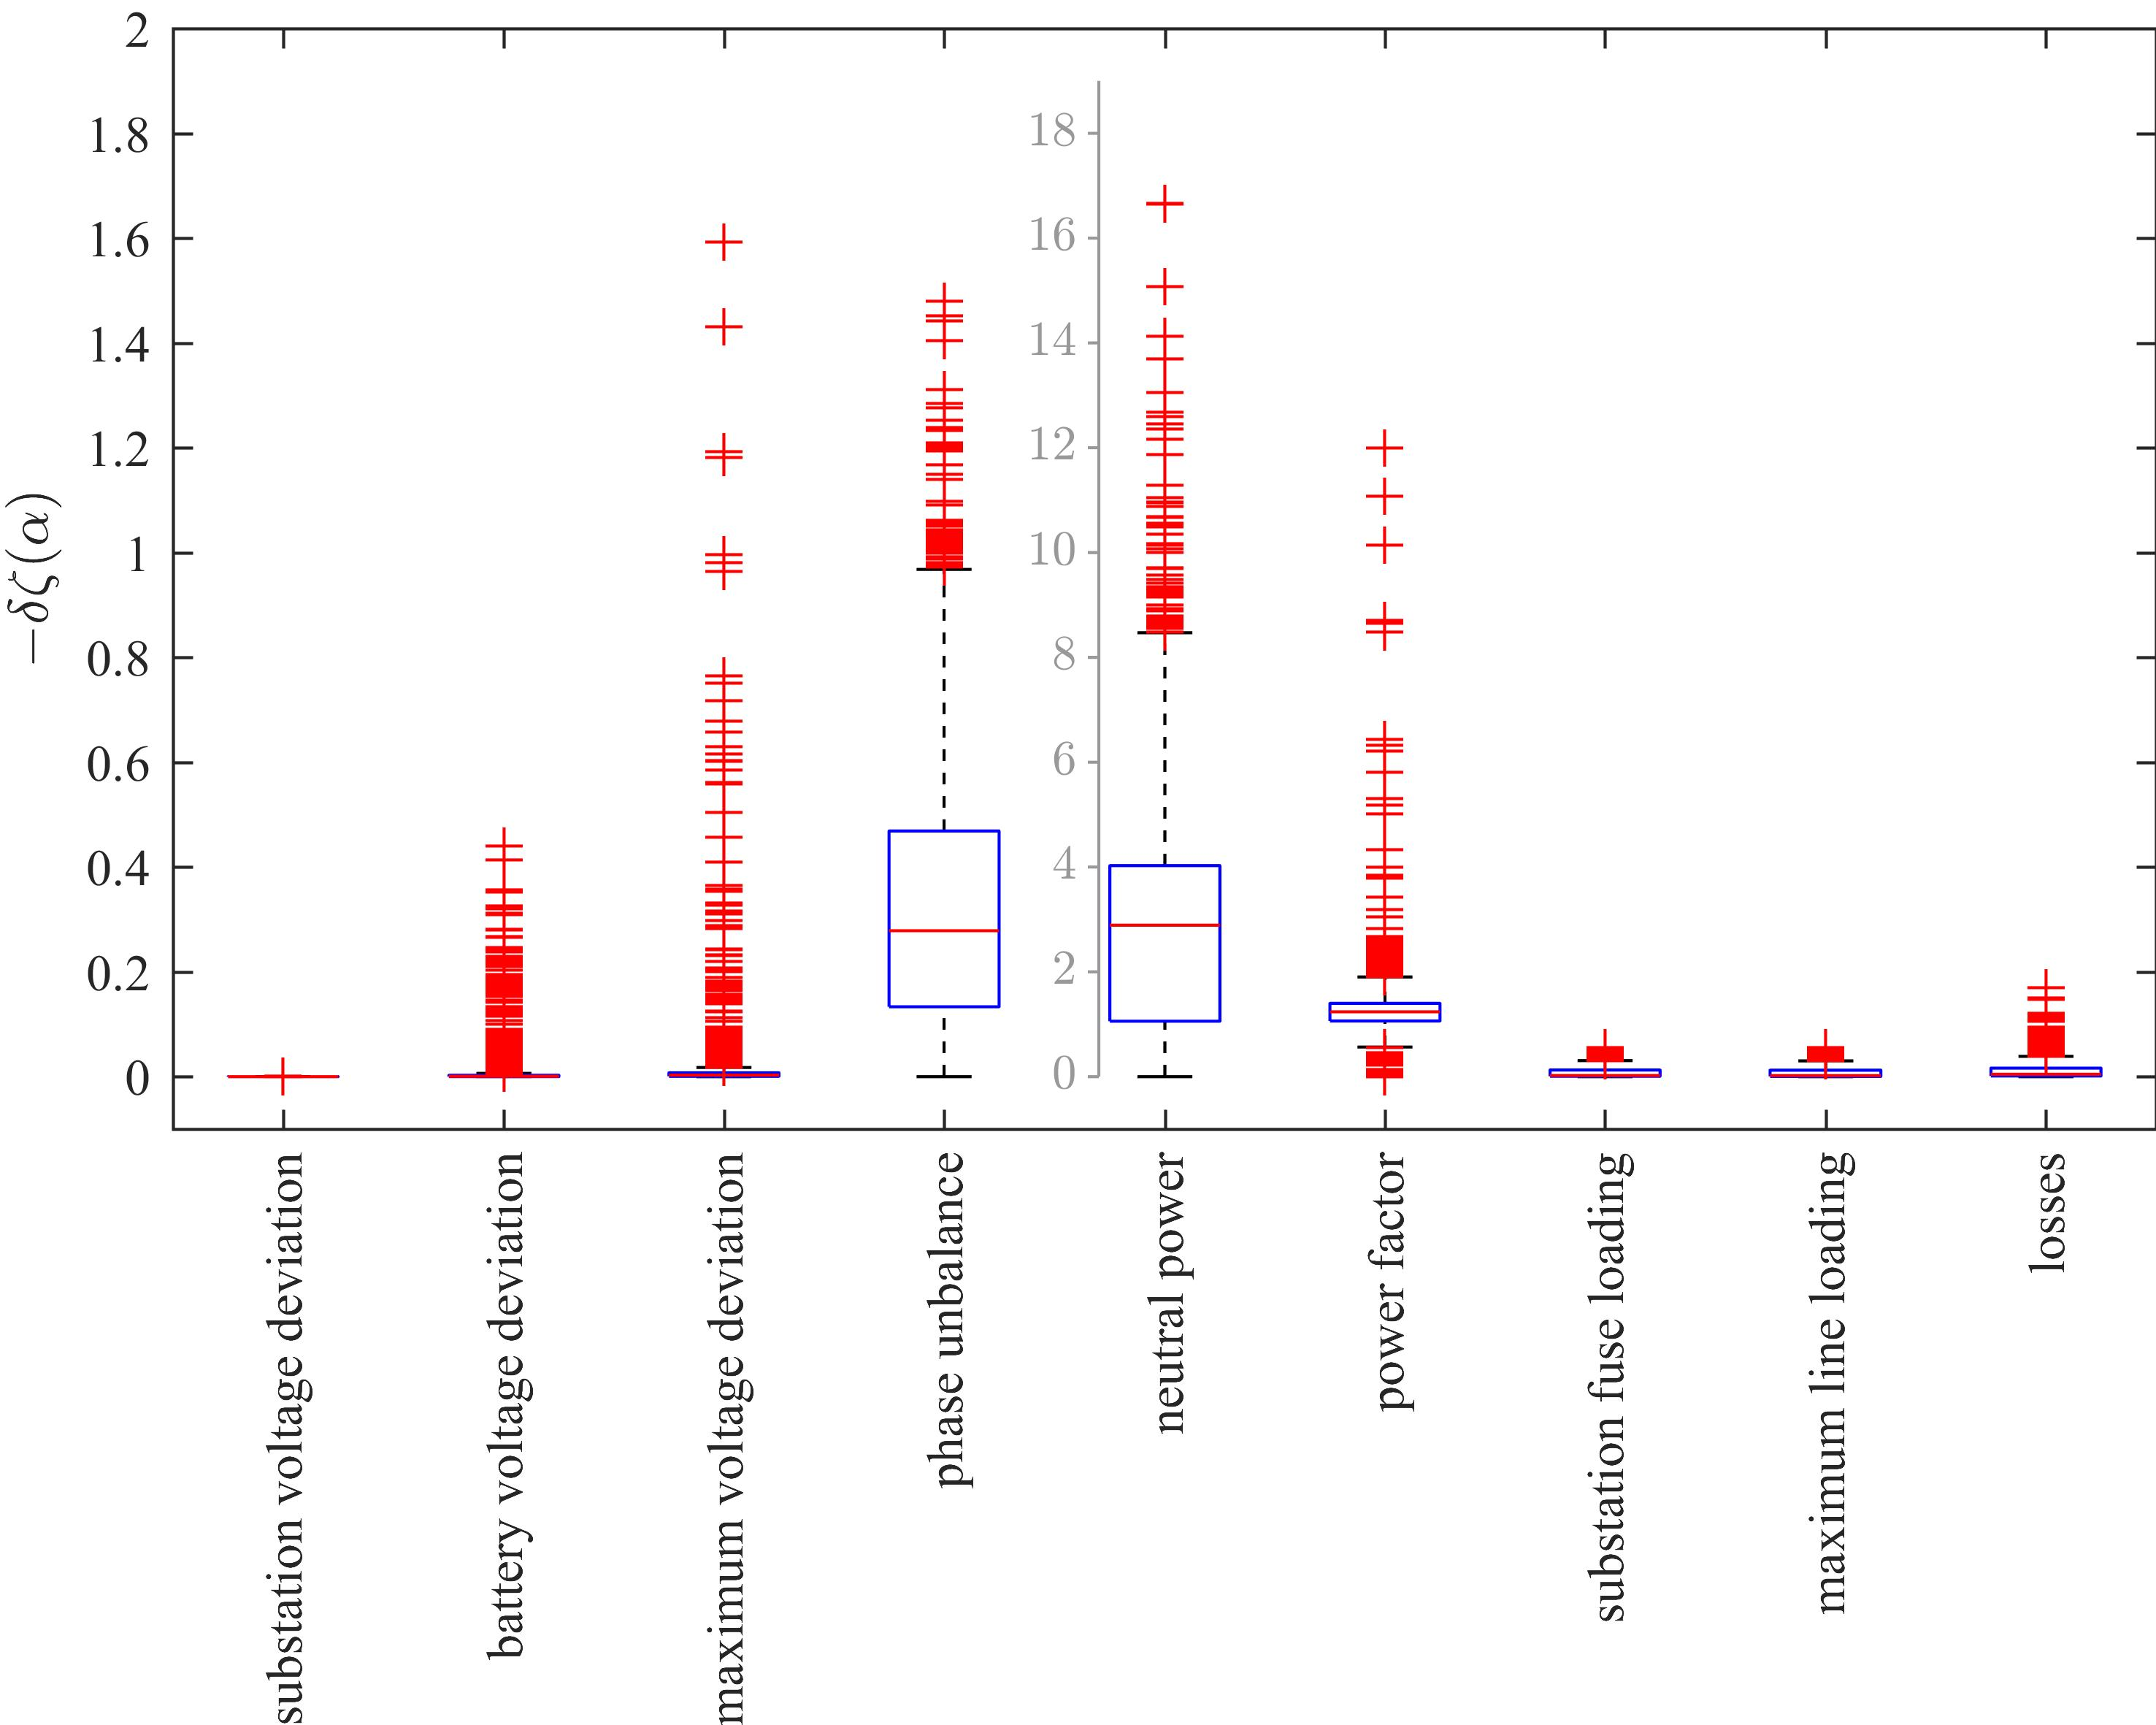
\includegraphics[width=\textwidth]{_chapter1/fig/results/boxplot-overall-improvements}
\caption{Cost-function improvement spread, when comparing against the normal ESMU operation case and when optimising for the underlying cost (a separate y-axis is introduced for the optimisation of ``neutral power'').}
\label{ch1:fig:boxplot-overall-improvements}
\end{figure}

This figure shows the how the reduction in cost (defined in Equation~\ref{ch1:equ:weighted-sum-cost-function}) is distributed.
In this case the cost reduction (i.e. $-\delta\zeta(\boldsymbol{\alpha})$) is the change in cost from the \textit{normal} ESMU operation case to \textit{minimisation} operation cases, for ``phase unbalance'' $\delta\zeta(\boldsymbol{\alpha}) = \zeta(\alpha_1 = 1) - \zeta(\alpha_6 = 1)$).
Due to the different scales however, the improvements are difficult to observe.
Therefore, this cost reduction has been normalised in regards to the \textit{normal} ESMU operation case and is replotted in Figure~\ref{ch1:fig:boxplot-relative-improvements}.

\begin{figure}\centering
	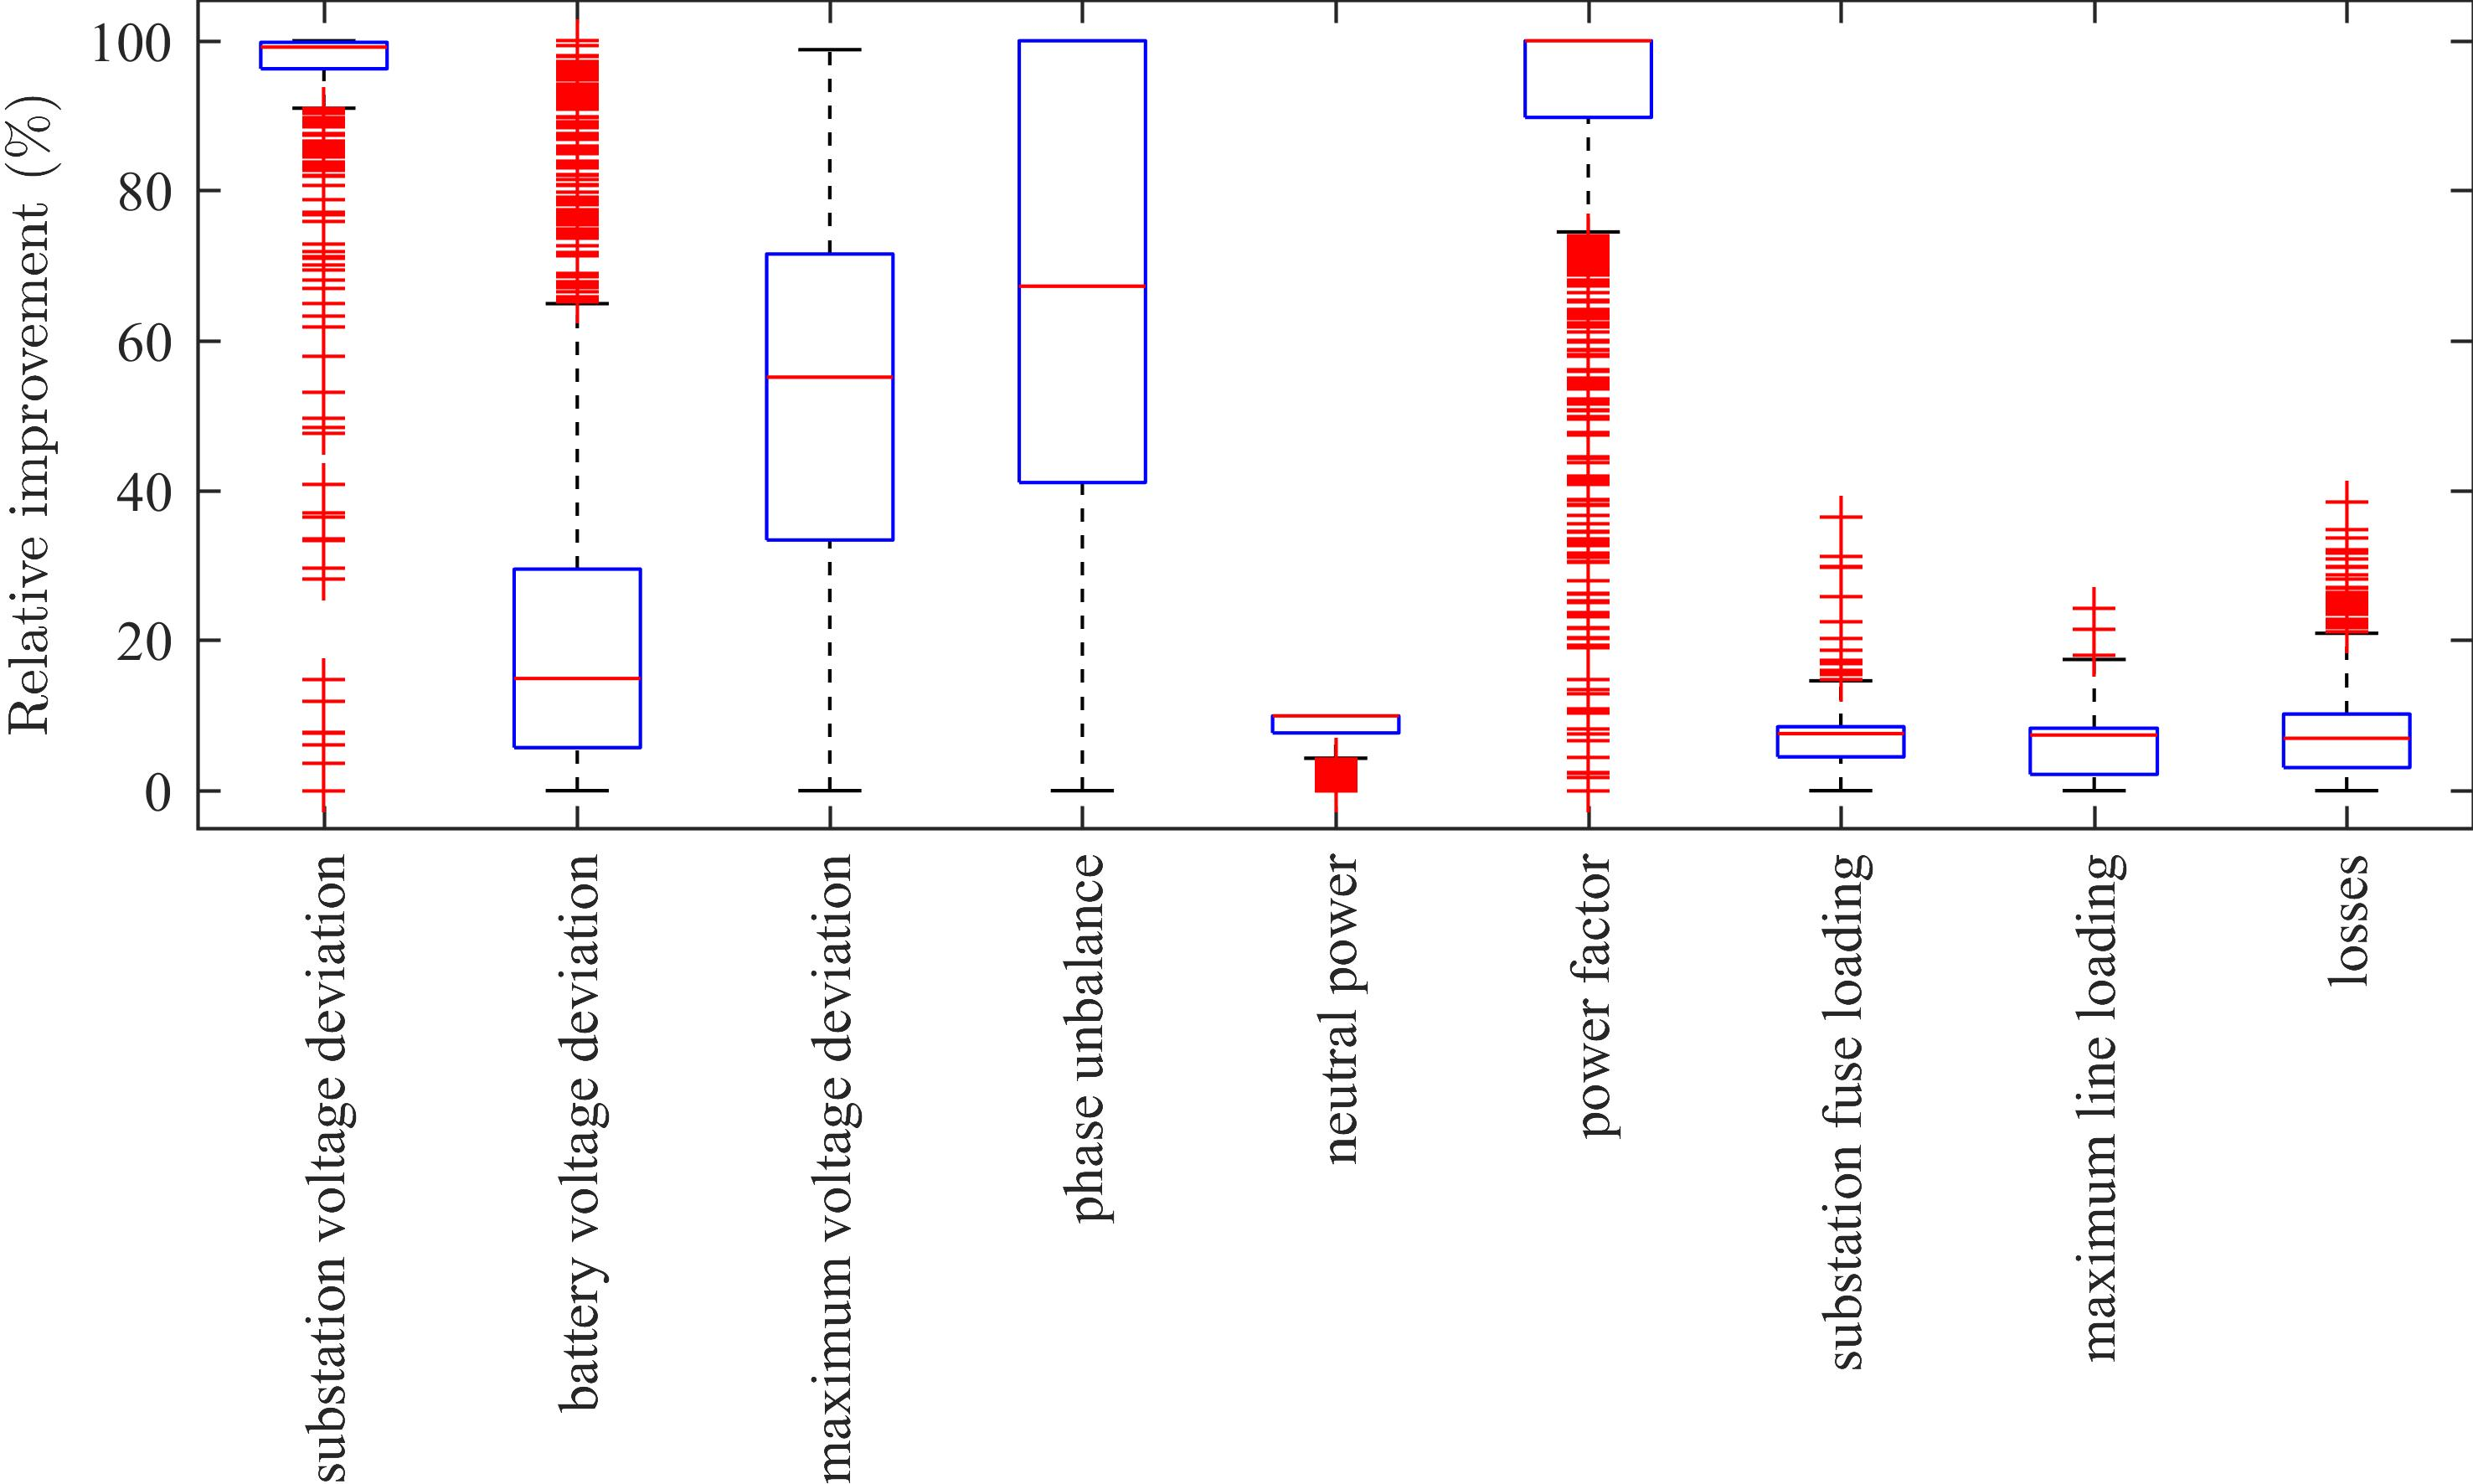
\includegraphics[width=\textwidth]{_chapter1/fig/results/boxplot-relative-improvements}
\caption{Relative cost improvement spread, when comparing against the \textit{normal} ESMU operation case and when optimising for the underlying cost.}
\label{ch1:fig:boxplot-relative-improvements}
\end{figure}

In this figure it can be seen that the most significant cost related impact on the network is yielded when improving voltage deviation, phase unbalance and power factor costs.
Reason for this noticeably larger impact is due to ESMU being able to assign its scheduled active power to all three phases in an optimal manner as long as the predetermined half-hourly schedule is obeyed.
It is this obedience constraint that limits the extend by which all other key network parameters can be impacted.
Reactive power on the other hand is only indirectly constrained by the ESMU schedule.
The only limit that applies to the ESMU's reactive power injection capabilities is the remaining PMU capacity after committing to the scheduled active power.
Also, unlike active power, reactive power has a smaller impact on the LV network due to its physical property (i.e. being more resistive than inductive).
Nonetheless, when each key network parameters became subject to their corresponding cost minimisation all of them were impacted positively.

In addition to the box-plots, the cost improvements (whose box-plots are presented in the Appendix~\ref{appx-a:ch1:additional-difference-analysis}), are calculated and tabulated in Table~\ref{ch1:tab:cost-table}.
This table shows the cumulative difference in $-\delta\zeta(\boldsymbol{\alpha})$ between the \textit{normal} case and the \textit{minimisation} case, i.e. where $\delta\zeta(\boldsymbol{\alpha}) = \zeta(\alpha_1 = 1) - \zeta(\alpha_2 = 1)$.
However, instead of only presenting the cost reduction that is yielded when minimising it this table also includes all other resulting costs, i.e. the daily aggregated cost to be precise.
This value is defined as the ``cumulative cost difference'', i.e. $\sum_t \delta\zeta(\boldsymbol{\alpha})$.
In addition to the comparison between \textit{minimisation} and \textit{normal} cases, the \textit{normal} case is compared to the \textit{base} case for reference.
For convenience all positive cost reductions (i.e. network improvements) have been highlighted.

\begin{sidewaystable}\centering
\definecolor{light_blue}{rgb}{0.9, 0.9, 1.0}
\definecolor{dark_blue}{rgb}{0.5, 0.5, 1.0}
\begin{tabular}{cc|ccccccccc|}
& & \multicolumn{9}{c}{minimisation cases} \\
& \rotatebox[origin=l]{90}{normal}& \rotatebox[origin=l]{90}{substation voltage deviation}& \rotatebox[origin=l]{90}{battery voltage deviation}& \rotatebox[origin=l]{90}{maximum voltage deviation}& \rotatebox[origin=l]{90}{phase unbalance}& \rotatebox[origin=l]{90}{neutral power}& \rotatebox[origin=l]{90}{power factor}& \rotatebox[origin=l]{90}{substation fuse loading}& \rotatebox[origin=l]{90}{maximum line loading}& \rotatebox[origin=l]{90}{losses} \\
\hline
\multicolumn{1}{r|}{substation voltage deviation} & 0.00 & \cellcolor{light_blue}0.08 & -2.49 & -1.39 & -4.89 & -8.72 & \cellcolor{light_blue}0.04 & 0.00 & \cellcolor{light_blue}0.01 & -1.09 \\
\multicolumn{1}{r|}{battery voltage deviation} & -5.01 & -0.40 & \cellcolor{light_blue}15.52 & \cellcolor{light_blue}17.04 & \cellcolor{light_blue}9.14 & \cellcolor{light_blue}14.93 & -2.85 & -0.43 & -1.62 & \cellcolor{light_blue}13.69 \\
\multicolumn{1}{r|}{maximum voltage deviation} & -6.83 & -1.15 & \cellcolor{light_blue}28.22 & \cellcolor{light_blue}36.42 & \cellcolor{light_blue}24.66 & \cellcolor{light_blue}33.05 & -3.07 & -0.56 & -2.57 & \cellcolor{light_blue}25.44 \\
\multicolumn{1}{r|}{phase unbalance} & \cellcolor{light_blue}12.15 & \cellcolor{light_blue}40.93 & \cellcolor{light_blue}284.87 & \cellcolor{light_blue}380.57 & \cellcolor{light_blue}490.22 & \cellcolor{light_blue}351.35 & \cellcolor{light_blue}40.66 & \cellcolor{light_blue}10.02 & \cellcolor{light_blue}5.03 & \cellcolor{light_blue}441.24 \\
\multicolumn{1}{r|}{neutral power} & -0.83 & -96.72 & \cellcolor{light_blue}2303.70 & \cellcolor{light_blue}1642.37 & \cellcolor{light_blue}2698.78 & \cellcolor{light_blue}4415.85 & \cellcolor{light_blue}319.23 & \cellcolor{light_blue}133.46 & \cellcolor{light_blue}53.53 & \cellcolor{light_blue}2401.12 \\
\multicolumn{1}{r|}{power factor} & -0.27 & \cellcolor{light_blue}159.42 & -7.63 & -37.25 & -633.30 & -314.11 & \cellcolor{light_blue}183.01 & \cellcolor{light_blue}145.35 & \cellcolor{light_blue}136.87 & \cellcolor{light_blue}88.84 \\
\multicolumn{1}{r|}{substation fuse loading} & \cellcolor{light_blue}5.14 & \cellcolor{light_blue}13.34 & -0.43 & -8.69 & -51.76 & -72.68 & \cellcolor{light_blue}14.37 & \cellcolor{light_blue}10.98 & \cellcolor{light_blue}10.91 & \cellcolor{light_blue}5.64 \\
\multicolumn{1}{r|}{maximum line loading} & \cellcolor{light_blue}4.53 & \cellcolor{light_blue}12.88 & -6.17 & -10.04 & -80.41 & -97.30 & \cellcolor{light_blue}13.89 & \cellcolor{light_blue}10.69 & \cellcolor{light_blue}10.94 & \cellcolor{light_blue}4.72 \\
\multicolumn{1}{r|}{losses} & \cellcolor{light_blue}4.34 & \cellcolor{light_blue}7.22 & \cellcolor{light_blue}13.38 & -4.46 & -46.37 & -66.32 & \cellcolor{light_blue}12.89 & \cellcolor{light_blue}9.65 & \cellcolor{light_blue}9.02 & \cellcolor{light_blue}17.13 \\
\end{tabular}
\caption{Cross-cost improvements due to adjustments to the original ESMU schedule.}
\label{ch1:tab:cost-table}
\end{sidewaystable}


As expected all entries along the diagonal are positive in cross-cost difference, i.e. where the evaluated cost is also the cost that was minimised.
But beside this fact one can also observe which cost minimisation has an impact on different costs.
For example, adjusting the ESMU schedule to achieve the largest reduction in distribution losses (i.e. far right column) improves nearly all key network parameters apart from substation voltage deviation.
Furthermore, Table~\ref{ch1:tab:cost-table} indicates that reducing battery voltage deviation, maximum voltage deviation, phase unbalance and neutral power (respectively, columns 3, 4, 5 and 6) have a noticeable impact on each other.
Minimising any of these four costs does however not impact power factor, loading and losses (apart from reducing battery voltage deviation).

Although the impact on network improvements for some costs is easily determined and explained with the underlying physical properties of distribution systems, other impacts of minimising cost do not share this transparency.
For example, minimising power factor (column 7) has a greater impact on reducing line loadings than directly minimising substation or maximum line loading (column 8 and 9, respectively).
The reason behind this effect is due to instantaneous apparent power contributing to the line current.
This means that maximising the network's power factor minimises reactive load which in turn lowers the total line current.
Since the solving algorithm does not know which cost to minimise first, the task of finding a global minimum becomes more difficult.
To improve the performance of adjusting ESMU powers one could propose to concatenate several cost minimisation procedures in a sequential series.
Doing so would focus the search for global minima for each iteration of the sequence, yet this lies outside the scope of this Thesis and can be continued in future research.

\subsection{Probability Density Analysis}
\label{ch1:subsec:probability-density-analysis}

The final part of analysing the results is to determine whether the cumulative cross-cost differences are statistically significant.
To do so, the probability density functions (PDF) of the cross-cost differences is analysed using a null hypothesis test.
The underlying data is conditioned in order to meet all prerequisites that are necessary to perform the null hypothesis test, like the standard $t$-test.
These prerequisites include stationarity, low auto-correlation and high gaussianity of the underlying time-series.
The procedure to meet these prerequisites is carried out without falsifying the data which means that all applied conditioning operations were restricted to time-series division and linear transformation.
Details on the exact data conditioning steps are outside the scope of this chapter, but for completeness they are included in Appendix~\ref{appx-a:ch1:probability-density-analysis}.

\begin{sidewaystable}\centering
\definecolor{light_blue}{rgb}{0.9, 0.9, 1.0}
\definecolor{dark_blue}{rgb}{0.5, 0.5, 1.0}
\definecolor{light_red}{rgb}{1.0, 0.5, 0.5}
\begin{tabular}{cc|ccccccccc|}
& & \multicolumn{9}{c}{minimisation cases} \\
& \rotatebox[origin=l]{90}{normal}& \rotatebox[origin=l]{90}{substation voltage deviation}& \rotatebox[origin=l]{90}{battery voltage deviation}& \rotatebox[origin=l]{90}{maximum voltage deviation}& \rotatebox[origin=l]{90}{phase unbalance}& \rotatebox[origin=l]{90}{neutral power}& \rotatebox[origin=l]{90}{power factor}& \rotatebox[origin=l]{90}{substation fuse loading}& \rotatebox[origin=l]{90}{maximum line loading}& \rotatebox[origin=l]{90}{losses} \\
\hline
\multicolumn{1}{r|}{substation voltage deviation} & $0.851$ & \cellcolor{light_blue}$<0.001$ & $0.999$ & $1.000$ & $0.999$ & $1.000$ & \cellcolor{light_blue}$<0.001$ & \cellcolor{light_blue}$<0.001$ & \cellcolor{light_blue}$<0.001$ & $0.999$ \\
\multicolumn{1}{r|}{battery voltage deviation} & $0.899$ & \cellcolor{light_blue}$<0.001$ & \cellcolor{light_blue}$<0.001$ & \cellcolor{light_blue}$<0.001$ & \cellcolor{light_blue}$<0.001$ & \cellcolor{light_blue}$<0.001$ & \cellcolor{light_blue}$0.022$ & \cellcolor{light_blue}$0.018$ & $0.325$ & \cellcolor{light_blue}$<0.001$ \\
\multicolumn{1}{r|}{maximum voltage deviation} & $0.718$ & \cellcolor{light_blue}$0.000$ & \cellcolor{light_blue}$<0.001$ & \cellcolor{light_blue}$<0.001$ & \cellcolor{light_blue}$<0.001$ & \cellcolor{light_blue}$<0.001$ & $0.086$ & $0.167$ & $0.772$ & \cellcolor{light_blue}$<0.001$ \\
\multicolumn{1}{r|}{phase unbalance} & $0.331$ & \cellcolor{light_blue}$<0.001$ & \cellcolor{light_blue}$<0.001$ & \cellcolor{light_blue}$<0.001$ & \cellcolor{light_blue}$<0.001$ & \cellcolor{light_blue}$<0.001$ & \cellcolor{light_blue}$<0.001$ & \cellcolor{light_blue}$0.001$ & \cellcolor{light_blue}$0.038$ & \cellcolor{light_blue}$<0.001$ \\
\multicolumn{1}{r|}{neutral power} & $0.940$ & $0.999$ & \cellcolor{light_blue}$<0.001$ & \cellcolor{light_blue}$<0.001$ & \cellcolor{light_blue}$<0.001$ & \cellcolor{light_blue}$<0.001$ & \cellcolor{light_blue}$<0.001$ & \cellcolor{light_blue}$<0.001$ & \cellcolor{light_blue}$0.016$ & \cellcolor{light_blue}$<0.001$ \\
\multicolumn{1}{r|}{power factor} & $0.488$ & \cellcolor{light_blue}$<0.001$ & \cellcolor{light_blue}$0.020$ & $0.999$ & $0.999$ & $1.000$ & \cellcolor{light_blue}$<0.001$ & \cellcolor{light_blue}$<0.001$ & \cellcolor{light_blue}$<0.001$ & \cellcolor{light_blue}$<0.001$ \\
\multicolumn{1}{r|}{substation fuse loading} & $0.777$ & \cellcolor{light_blue}$<0.001$ & $0.929$ & $0.999$ & $0.999$ & $1.000$ & \cellcolor{light_blue}$<0.001$ & \cellcolor{light_blue}$<0.001$ & \cellcolor{light_blue}$<0.001$ & \cellcolor{light_blue}$0.001$ \\
\multicolumn{1}{r|}{maximum line loading} & $0.846$ & \cellcolor{light_blue}$<0.001$ & $0.996$ & $0.999$ & $0.999$ & $0.999$ & \cellcolor{light_blue}$<0.001$ & \cellcolor{light_blue}$<0.001$ & \cellcolor{light_blue}$<0.001$ & $0.102$ \\
\multicolumn{1}{r|}{losses} & $0.881$ & \cellcolor{light_blue}$<0.001$ & \cellcolor{light_blue}$<0.001$ & $0.637$ & $0.910$ & $0.999$ & \cellcolor{light_blue}$<0.001$ & \cellcolor{light_blue}$<0.001$ & \cellcolor{light_blue}$<0.001$ & \cellcolor{light_blue}$<0.001$ \\
\end{tabular}
\caption{$p$-values for statistical evidence of cross-cost improvements based on statistical two-sample single-tailed $t$-test.}
\label{ch1:tab:t-test-table}
\end{sidewaystable}


Table~\ref{ch1:tab:t-test-table} presents the results from this analysis, where $p$-values have been tabulated and those cells with a value below $0.05$ have been highlighted.
A similar pattern to that in the previous table can be seen (i.e. Table~\ref{ch1:tab:cost-table}).
In this table however, instead of just comparing cross-cost reductions, statistical indications to support the significance of the findings is presented.
In combination with the preceding table one can therefore determine that the impact of optimising operation based on maximum voltage deviation has little to no significant impact on improvements in power factor whilst adjusting ESMU powers to improve the network's power factor has the most significant statistical impact on the chosen key network parameters.
